% The document class supplies options to control rendering of some standard
% features in the result.  The goal is for uniform style, so some attention 
% to detail is *vital* with all fields.  Each field (i.e., text inside the
% curly braces below, so the MEng text inside {MEng} for instance) should 
% take into account the following:
%
% - author name       should be formatted as "FirstName LastName"
%   (not "Initial LastName" for example),
% - supervisor name   should be formatted as "Title FirstName LastName"
%   (where Title is "Dr." or "Prof." for example),
% - degree programme  should be "BSc", "MEng", "MSci", "MSc" or "PhD",
% - dissertation title should be correctly capitalised (plus you can have
%   an optional sub-title if appropriate, or leave this field blank),
% - dissertation type should be formatted as one of the following:
%   * for the MEng degree programme either "enterprise" or "research" to
%     reflect the stream,
%   * for the MSc  degree programme "$X/Y/Z$" for a project deemed to be
%     X%, Y% and Z% of type I, II and III.
% - year              should be formatted as a 4-digit year of submission
%   (so 2014 rather than the accademic year, say 2013/14 say).

\documentclass[ % the name of the author
author={Dillon Keith Diep},
% the name of the supervisor
supervisor={Dr. Carl Henrik Ek},
% the degree programme
degree={MEng},
% the dissertation    title (which cannot be blank)
title={ART-CG:},
% the dissertation subtitle (which can    be blank)
subtitle={Assisted Real-time Content Generation of 3D Hair by Learning Manifolds},
% the dissertation     type
type={Research},
% the year of submission
year={2017} ]{dissertation}
\begin{document}
% =============================================================================

% This section simply introduces the structural guidelines.  It can clearly
% be deleted (or commented out) if you use the file as a template for your
% own dissertation: everything following it is in the correct order to use 
% as is.

% =============================================================================

% This macro creates the standard UoB title page by using information drawn
% from the document class (meaning it is vital you select the correct degree 
% title and so on).

\maketitle

% After the title page (which is a special case in that it is not numbered)
% comes the front matter or preliminaries; this macro signals the start of
% such content, meaning the pages are numbered with Roman numerals.

\frontmatter

% This macro creates the standard UoB declaration; on the printed hard-copy,
% this must be physically signed by the author in the space indicated.

\makedecl

% LaTeX automatically generates a table of contents, plus associated lists 
% of figures, tables and algorithms.  The former is a compulsory part of the
% dissertation, but if you do not require the latter they can be suppressed
% by simply commenting out the associated macro.

\tableofcontents
\listoffigures
\listoftables
\listofalgorithms
\lstlistoflistings

% The following sections are part of the front matter, but are not generated
% automatically by LaTeX; the use of \chapter* means they are not numbered.

% -----------------------------------------------------------------------------

\chapter*{Executive Summary}
Production of 3D virtual worlds is a time-consuming and costly process that also demand expert knowledge. 3D assets encompass a vast range of applications, ranging from simulations and research to contributing towards the functioning of many industries. Our proposition of probabilistic non-linear dimension reduction consolidates observed variables to provide a parsimonious collection of latent variables, drastically diminishing the complexity of the production pipeline. Simplifying a procedure within the pipeline yield increased throughput and offer an opportunity for rapid prototyping. A non-linear approach minimises loss of information; thus high dimensional data can be reduced effectively to dimensionality that is sufficiently low. Non-experts may find directing a few descriptive components within a low dimension representation easier than controlling an overwhelming number of attributes present in the original data.

One particular task is the creation of 3D hair geometry for humanoid characters. Creating 3D hair is arduous as hair structure is a complex system containing much interdependence between components. The properties of 3D hair geometry pose significant challenges for machine learning solutions. Machine learning typically uses large data sets for training on problems that often have a concise answer for a given prediction. The application of machine learning to enhance production for creative work is an exciting field that faces novel challenges: artistic products tend to have small sets of data available, and evaluation of quality is subjective. Given the same input, acceptable solutions can vary significantly. The outlined peculiarities of applying machine learning to 3D mesh data establish a unique field of problems to investigate.

Existing tools for 3D modelling have remained mostly static in the paradigm of approach over the past several decades. Automation through methods such as procedural generation can produce content faster. However, the lack of control over the final result causes standard automation to be typically less desirable than traditional methods of 3D modelling. The research hypothesis of this study is that of applying non-linear probabilistic dimensionality reduction to improve the efficacy of creative content production for exceptionally high dimensional data such as complex 3D hair geometry on virtual humanoids.

\begin{quote}
	Deliverables:
	\begin{itemize}
		\item Formulating a generative model for 3D humanoid hair structure.
		\item Resolving the alignment problem by repairing raw input mesh data and feature extraction by approximating parameters of our generative model.
		\item Learning a low dimension latent-space of high dimensional hair structure data.
		\item Investigated the performance of various kernels and its impact on the latent variable model.
		\item Implemented an add-on package for a 3D production program, Blender.
		\begin{itemize}
			\item Generating guiding hair splines from the output of our regression model.
			\item Developed with a small training set that is practical for content creators.
			\item Achieving real-time performance, matching state of the art non-learning tools.
			\item Including functionality to records user activity for analysis.
		\end{itemize}
		\item Evaluation of data collected from survey and tests.
	\end{itemize}
\end{quote}

% -----------------------------------------------------------------------------

\chapter*{Supporting Technologies}

\begin{quote}
	\noindent
	\begin{itemize}
		\item Python with standard libraries for implementation.
		\item GPy library to implement the regression model.
		\item NumPy, SciPy, and Networkx for operations and processing meshes.
		\item PIL, Matplotlib, and Plotly for plotting images and graphs.
		\item Pickle for serialising objects as files.
		\item Blender API for mesh processing and the Blender 3D program for demonstration of our regression model.
		\item Google Forms to create feedback survey.
	\end{itemize}
\end{quote}

% -----------------------------------------------------------------------------

\chapter*{Notation and Acronyms}

\begin{quote}
	\noindent
	\begin{tabular}{lcl}
		$x$                 &:	& Scalar\\
		$\bm{x}$            &:	& Column vector\\
		$\bm{x}^T$			&:	& Row vector, superscript T denotes transpose\\
		$x_i$               &:  & the $i$-th value of a vector $\bm{x}$\\
		$\bm{I}$ 			&:	& Identity matrix\\
		$\bm{X}\in \Re^{n \times m}$	&:	& Matrix of real numbers with size $n \times m$\\
		$\mathcal{N}\sim(\mu, \sigma^2)$ 			&:	& Gaussian (normal) distribution with mean $\mu$ and variance $\sigma^2$.\\
		DR					&:	& Dimensionality Reduction\\
		PCA		 			&:	& Principal Component Analysis\\
		GP-LVM	 			&:	& Gaussian Process Latent Variable Model\\
	\end{tabular}
\end{quote}

% -----------------------------------------------------------------------------

\chapter*{Acknowledgements}
I would like to thank coffee

% =============================================================================

% After the front matter comes a number of chapters; under each chapter,
% sections, subsections and even subsubsections are permissible.  The
% pages in this part are numbered with Arabic numerals.  Note that:
%
% - A reference point can be marked using \label{XXX}, and then later
%   referred to via \ref{XXX}; for example Chapter\ref{chap:context}.
% - The chapters are presented here in one file; this can become hard
%   to manage.  An alternative is to save the content in seprate files
%   the use \input{XXX} to import it, which acts like the #include
%   directive in C.

\mainmatter

% -----------------------------------------------------------------------------

\chapter{Contextual Background}
\label{chap:context}
This dissertation explores assisted real-time content generation through training regression models using unsupervised machine learning for the production of 3D hair geometry.
The purpose of a 3D object is to describe a surface. Typically we define geometric surfaces using a combination of many primitive components. The craft of 3D content is a meticulous procedure as content creators are required to work with enormously high dimensional observed data.
The objective of this project is to demonstrate the potential of probabilistic non-linear dimensionality reduction on creative content production by presenting a framework that improves the efficacy of producing 3D hair geometry. 
In this chapter, we will introduce complications of producing 3D hair geometry with traditional methods and past research on machine learning applied to creative fields. We will also outline the motivation and significance for research, including challenges and central objectives of this study.

\section{Production of 3D Content}
There are multiple representations of 3D objects in computer graphics. One way to obtain 3D geometry data is to sample surfaces of the physical world with a 3D scanner. Common representations of sampled geometric data include point clouds, range maps, and voxels. Such representations are effective for sampling as they reconstruct a surface from allocating many simple components.

\begin{figure}[!h]
	\centering
	%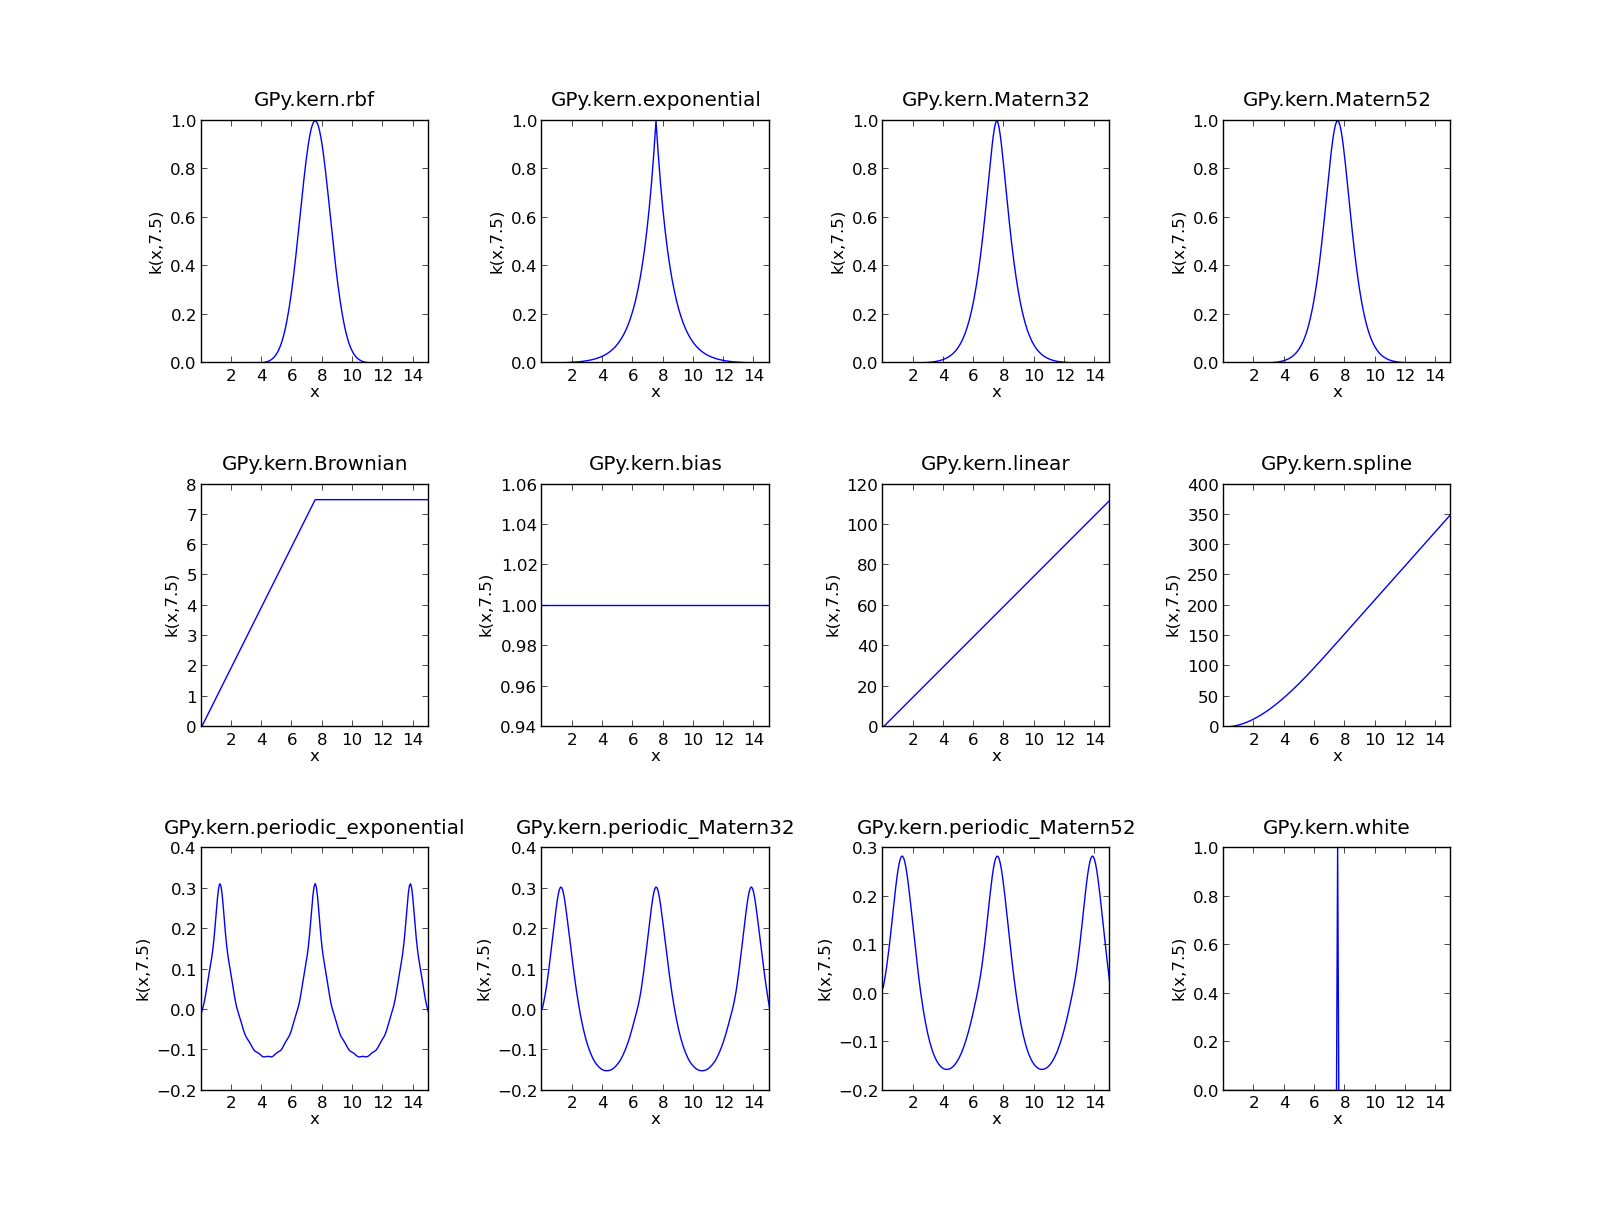
\includegraphics[scale=0.3]{images/gpyKernels}\\
	\caption{A point cloud representation is a collection of points (vertices) that describe surface geometry. Range images map pixels of a depth image to a set of points in the scene. Voxels are unit cubes, corresponding to the concept of pixels, a collection of voxels describe an object volumetrically.}
\end{figure}

Representations have advantages and disadvantages depending on the use case. It is possible to convert between representations; however, converting between representations may incur data loss. Precise representations are often mathematical models such as \textit{NURBS} (Non-Uniform Rational Basis Spline) - frequently applied in the \textit{CAD} (Computer-Aided Design) industry. Mathematical models are precise as they do not suffer from floating-point inaccuracy that is present in many representations. The most widely applied representation for \textit{CGI} (Computer-Generated Imagery) is \textit{polygonal meshes}. In a production environment, it is preferred to define geometry specifically to requirements of the design as opposed to capturing examples. Polygon meshes are simple to define, yet with established techniques such as UV texturing and normal mapping, are sufficiently expressive for visual purposes. A significant amount of study has been conducted in the field of polygon meshes to improve its versatility. The study of polygonal meshes is deeply rooted in computer graphics.

The elements of a polygonal mesh are \textit{vertices}, \textit{edges}, and \textit{faces}. The \textit{topology} of a mesh concerns with the arrangement of its components, well-organised topology is required to maintain geometric qualities when performing algorithmic operations on a mesh. In practice, professionals create polygon meshes with majority quad-face topology (faces formed from four edges) during production. The rendering pipeline often automatically converts polygon meshes to triangle faces (formed from three edges) as an optimisation process. \textit{Quadrilateral mesh} form ring loops that we call \textit{edge loops} which can be used to define the structure of geometry, thus conform better with editing tools and algorithms than \textit{triangle meshes}.

State of the art 3D production software such as AutoDesk Maya, 3DS Max, and Blender are advanced programs with a sophisticated list of features. That said, such programs have extremely convoluted user interfaces, even the most experienced professionals do not recognise each and every tool available. The high learning curve with an overwhelming user experience is not beginner-friendly. In fact, the most functionality is only accessible through an API (Application Program Interface) via a scripting language.  Experienced users welcome this complexity as it allows creators to customise their ideal workflow, but it also creates a high barrier to entry for non-experts who wish to possess the capability of such 3D programs.

\subsection{3D Hair Geometry}
In recent years, leading solutions for real-time simulation of realistic hair and fur, such as \textit{NVIDIA HairWorks} and \textit{AMD TressFX} has emerged. These solutions, however, have limited application in comparison to their traditional counterpart of polygonal hair. It is often the case that texture-mapped polygonal hair is used as a fallback when advanced simulation fails. Realism is not necessarily always desirable, and polygon hair can flexibly represent different art styles. In some cases, a blend of multiple representations is used to balance between cost and quality. 3D hair in cinematography with a large budget can afford to render hair with much higher fidelity for major characters, but would still consider using efficient variants for scenarios such as crowd simulation. Ultimately, we can observe that the representation of virtual hair follows a structure of splines with control points that define the overall organisation of strands or segments. This information will allow transferral between representations to an extent.

On average, a human is born with between 90,000 to 150,000 scalp hair follicles \cite{hairfollicles}. It is computationally very expensive to render and animate physically correct hair, but creative liberties are taken to approximate or stylise 3D hair such that it is both acceptable aesthetically and feasible regarding performance. This study considers modelling of hair geometry, the motion of hair is assumed to be its default resting pose.

\begin{figure}[!h]
	\centering
	To add %*
	\caption{Image of hair geometry.}
\end{figure}

There are various ways to construct a polygonal hair mesh. We are concerned with hair meshes formed from multiple planar sub-meshes of hair locks or segments. This type of hair mesh can express a variety of styles but produce densely arranged geometry. 
Producing hair mesh data is challenging as content creators manipulate data that is exceptionally high dimensional, this reflects on \textbf{the curse of dimensionality}, a term coined by Bellman \cite{curseofdyn} which refers to the phenomena where exhibited complexity of high-dimensional spaces grows exponentially greater than those of low-dimensionality. There are two perspectives where the curse of dimensionality applies in our project. First, from the viewpoint of a 3D content creator, appending data points to geometry on a 3D program becomes increasingly difficult. Tightly positioned components are laborious for creators to find or select, with each action having less impact on the overall surface. The other perspective is that of algorithmic complexity. Machine learning methods scale and generalise better when using a few key features, use of many features is computationally expensive and risks overfitting.

Procedural generation techniques produce output that adheres to rules established by the generative model defined. Generation of terrains and city modelling sometimes employ procedural techniques to take advantage of its systematic nature to mass produce variations in agreement with specified patterns\cite{procedural1}. Fractals and methods such as the Lindenmayer system have been used to create patterns that resemble those observed in nature\cite{lsystem}. Automated techniques such as the ones discussed, however, are seldom used for modelling distinct objects with a specific design. It is an involved process to control the output of procedurally generated content without heavily restricting its capabilities. Automated methods that do not learn cannot adapt to changing demands without reimplementation.

\section{Related Research of Machine Learning in Creative Fields}
Three major paradigms divide the task of machine learning:
\begin{itemize}
	\item \textit{Supervised learning} is provided input training examples with desired outputs to learn the mapping of inputs to an output.
	\item \textit{Unsupervised learning} seeks to learn the structure of and relation between input data.
	\item \textit{Reinforcement learning} iteratively improve a pool of solutions by simulating an environment that applies concepts inspired by the theory of evolution.
\end{itemize}
The role that learning methods play in both manufacturing and consumer application continue to grow, however, adoption has been slow for creative fields.  Generally, robust models improve in performance as more reliable data is obtained. Creative production values uniqueness and versatility, properties that cause difficulty in machine learning methods. Varying artistic styles in design complicate feature analysis and ambiguity of correctness is problematic when predicting an output. In machine learning, prediction of continuous variables is a \textbf{regression} problem. 

Style-based inverse kinematics introduced the Scaled Gaussian Process Latent Variable Model to learn the probabilistic distribution of a 3D human posture model\cite{styleik}. Character posing from motion data is represented as a 42-dimensional feature vector that encapsulated joint information of a humanoid body. Learning a model of poses established the relation between joints and identified constraints exhibited in the training data - where unusual postures are given a lower likelihood rating.

A latent doodle space is the use of a low-dimension latent space that has been applied on simple line drawings\cite{latentdoodle}. The motivation of a latent doodle space is to generating new drawings that are inspired by the input data. There are two key phases to derive a latent doodle space: the first challenge is to identify line strokes within drawings, a latent variable method is then used to learn a latent space.

A study by Campbell \& Kautz presented a framework that learns the latent manifold of existing font styles\cite{fontmanifold}. The process involved universal parametrization of fonts to a polyline representation so that a distance measure is applicable and the generative model can interpolate between styles. Unsupervised learning with the GP-LVM model enabled rapid prototyping and non-experts could create font styles without experience on type design.

Drawing assistance powered by large-scale crowd-sourcing explored the potential of data driven drawing to prompt for correction by achieving an artistic consensus\cite{drawingassistance}. A consensus is found by learning a correction vector field from training drawings. Stroke-correction is applied using the correction vector field to adjust user input dynamically.

Chai et al. introduced AutoHair, a method for automatic modelling of 3D hair from a portrait image\cite{autohair}. The approach extracts information from images and uses a database of hair meshes to construct a 3D representation of the information conveyed. A hierarchical deep neural network trained on annotated hair images learn to segment hair and estimate growth direction within portraits. Data-driven hair matching and modelling algorithm fit meshes from the database to parameters output by the neural net model to automatically produce 3D hair. The experiment developed a traversable hairstyle space of 50,000 hair models, using training images and 3D exemplars obtained from the internet.

Research regarding creative content often parametrise the input data so that machine learning is applicable. There is no clearly defined solution for a problem in the creative field, effective solutions strive for versatility, employing consensus decision making or offering multiple solutions. To overcome the challenges introduced, dimensionality reduction through unsupervised learning with probabilistic latent variable models such as the Gaussian Process Latent Variable Model (GP-LVM) \cite{gplvm} present an opportunity to learn stylistic properties of design and predict multiple acceptable outputs by analysing the likelihood.

\section{Motivation and Significance}
Virtual hair creation is a necessity for characters of CG movies and video games that are embedded within culture both economically and as entertainment. Specialised artists learn to be proficient with the design of hair, variety of styles, and techniques for creation. In comparison to other forms of surfaces, hair meshes are densely concentrated, containing many data points that are exhausting to edit. Maintaining topology and issues such as overlapping surfaces are problematic among detailed meshes. Experienced artists might search for an existing base mesh that is similar to start on, but it is not always the case that such a base mesh exists - there are also concerns for quality, such as poor topology. Each alteration makes less impact as the geometry becomes more detailed and well-defined. The space of sensible changes become smaller. Design and production of 3D geometry remain a slow and delicate process.

Non-linear dimensionality reduction models are attractive candidates to resolve difficulties imposed by high dimensional data such as 3D polygonal hair geometry. That said, the process of machine learning is more involved than simply inputting training data into a model. In practice, data acquired are frequently encoded in complicated structures. Such data is seldom useful in its original form; feature extraction may be required to find an orderly representation that helps facilitate the learning stage. 3D meshes are complicated data structures that are heavily ambiguous when interpreting its data values without visualising the geometry. A motivational point for this project is to demonstrate how dimensionality reduction can be employed to tackle a real world problem such as content production.

Learning the relation of hair structure allows the potential of discovering new hairstyles.  It can also be used to output base geometry that fits the target output better than existing geometry available. Generative methods could ensure a level of quality, a clean topology that fits established specifications. The application of machine-learning based tools enhance the workflow of professional users and improve the experience for non-expert consumers. Such tools integrate into the production environment to improve the efficiency of acquiring initial base geometry and visually compare designs during pre-production. Non-expert users receive the ability to produce 3D geometry without requiring to learn the intrinsics of traditional 3D modelling software. The rise of augmented reality and 3D printing inspires the development of generative tools that are intuitive and simplistic to use. Applications that allow users to create personal content could also integrate machine-learning systems such as probabilistic regression models to prevent inappropriate or undesirable creation from being produced while providing options that surpass existing alternatives. Assisted content generation using machine learning can provide a convenient, non-intrusive and intuitive method for rapidly generating new hair geometry from existing data.

\section{Challenges}
This study faces multiple challenges. Firstly, 3D meshes are difficult to compare. The training data in its raw form will have varying dimensions. We can view meshes as samples of the actual surface. Thus meshes that represent the same object could differ drastically in the number of data points depending on its level of detail. Typical feature extraction methods do not work well on meshes as artistic products are sensitive to data loss - any change could affect the perception of final result drastically.

Another problem encountered is the lack of training data. Typical machine learning solutions use huge data sets in the order of hundreds of thousands for training, but for 3D meshes, the standard size of readily available training data is much smaller. Public repositories of 3D polygonal hair ordinarily contain up to thousands of meshes\cite{tsr}. Studios that store and organise past production may match the extent of public repositories, depending on the size of the company. Private repositories of independent artists will rarely exceed the order of hundreds.

The application of machine learning methods must also account for the subjectivity of evaluating artistic assets. The range of acceptable solutions is ambiguous, likened to how hair styles of characters can change drastically during the design phase.

In a production environment, the time required for a technique to return observable result directly affects throughput. For practical usage of assisted content generation, the technique should be reasonably fast in presenting observable output.

\section{Central Objectives}
%The aim of this study is ...
\begin{itemize}
	\item Resolving the alignment problem of 3D data through a representative generative model.
	\item Explore the application of non-linear dimension reduction for high dimensional data such as 3D hair geometry.
	\item Investigate the use of latent variables for identifying stylistic properties of 3D content.
	\item Demonstrate the use of a non-linear manifold to generate new hairstyles from training data.
	\item Enable an intuitive method for non-experts to easily create 3D hair geometry.
	\item Observable output demand performance comparable to real-time for practical use.
\end{itemize}

% -----------------------------------------------------------------------------

\chapter{Technical Background}
\label{chap:technical}
In the previous chapter we briefly introduced the \textit{curse of dimensionality}. High dimensional data is often counter-intuitive to perceive and process. Unfortunately, it is common for observed data to be in a representation of greater dimensionality than it requires. This gives rise to the notion of \textbf{dimensionality reduction}, a sub-field of machine learning that is motivated find a descriptive low-dimensional representation of data.
This chapter will establish the technical foundation required for understanding the probabilistic non-linear dimensionality reduction model we use for assisted real-time content generation of polygonal hair. Starting with principal component analysis (PCA), we review its probabilistic equivalent that contributes to the derivation of the Gaussian Process Latent Variable Model (GP-LVM). Then, we give a formal definition of polygon meshes from the perspective of graph theory - along with concepts that are useful for mesh processing.

\section{Principal Component Analysis}
In multivariate analysis, principal component analysis (PCA) is a statistical technique used to perform linear dimensionality reduction. It was originally introduced by Pearson \cite{pca1901}, and independently developed by Hotelling \cite{pca1933}, where the standard algebraic derivation of PCA was presented.

Consider the properties that describe hair structure. Observable variables that can be measured include location, orientation, length, and colour. The data collected may indicate that some variables change together, this relation is measured as the covariance. The PCA technique searches for an ordered set of principal components that retain maximal variance. A principal component can be viewed as a combination of the observed variables. Should two observed variables strongly covary linearly, then it is plausible to describe the data with a single variable instead. The more linearly observed variables covary, the less information is lost from choosing a smaller set of principal components, thus effectively reducing dimensionality.

Given a set of $n$ observed $d$-dimensional data represented as a design matrix, $\bm{X=[x_1,...,x_n]}^T$, the $q$ principal components $\bm{w_j}$, $j \in {1,...,q}$, are the orthonormal axes with maximal variance retained. The first principal component is a linear function $\bm{\alpha}^T_1\bm{X}$ that retains most variance of $\bm{X}$, where $\bm{\alpha} = [\alpha_{11}, \alpha_{12}, ..., \alpha_{1n}]$ is a vector of $n$ constants such that:
$$\bm{\alpha}^T_1\bm{X}=\alpha_{11}\bm{x_1}+\alpha_{12}\bm{x_2}+...+\alpha_{1n}\bm{x_n} = \sum^n_{i=1}a_{1i}\bm{x_i}$$
The following principal components are found by looking for a linear function that is orthogonal to the selected principal components and retain maximum variance.

PCA can be performed by singular value decomposition (SVD) of $\bm{X}$ in matrix form \cite{pca2002},
$$\bm{X=ULV}^T,$$
where given $r = r(\bm{X})$ denotes the rank of $\bm{X}$, then
$\bm{U} \in \Re^{n \times r}$ is a matrix of orthonormal columns that are the left singular vectors,
$\bm{L} \in \Re^{r \times r}$ is a diagonal matrix of the singular values of $\bm{X}$, and
$\bm{V} \in \Re^{d \times r}$ is a matrix of orthonormal columns that are the right singular vectors.

A limitation of standard PCA is the lack of a probabilistic solution. 
It is very likely for there to be a multiple sets of principal components that is equally acceptable. In the case of polygonal hair production, this aspect is more prominent as an artistic environment desires to evaluate various plausible designs. A probabilistic model will enable exploration of other stylistic embeddings for hair structure. One way to formulate a probabilistic model is to introduce the notion of noise among observed variables.

\section{The Gaussian Distribution}
The Gaussian (normal) distribution is a reasonable prior assumption for data that is subject to the central limit theorem, which states that as the sample size of a population tends to infinity, the distribution becomes increasingly Gaussian\cite[p.78]{bishop}.
A random variable $X$ that is normally distributed with mean $\mu$ and variance $\sigma^2$ is denoted as
$$X\sim\mathcal{N}(\mu, \sigma^2).$$
The Gaussian density for a single variable $y$ is expressed as\cite[p.78]{bishop}:
$$\mathcal{N}(y|\mu, \sigma^2)=\frac{1}{\sqrt{2\pi\sigma^2}}\exp\left(-\frac{(y-\mu)^2}{2\sigma^2}\right),$$
$$\mathcal{N}(y|\mu,\sigma^2) \equiv p(y|\mu,\sigma^2).$$
Notable properties of the Gaussian distribution that are useful include the summation (\ref{gd:sum}), scaling (\ref{gd:scale}), and product (\ref{gd:prod}) operation - all of which yields a result that is also a Gaussian distribution\cite[p.200]{gp}.
\begin{equation} \label{gd:sum}
\sum^n_{i=1}y_i\sim\mathcal{N}(\sum^n_{i=1}\mu_i,\sum^n_{i=1}\sigma^2_i)
\end{equation}

\begin{equation} \label{gd:scale}
wy\sim\mathcal{N}(w\mu,w^2\sigma^2)
\end{equation}

\begin{equation} \label{gd:prod}
\mathcal{N}(\bm{x|a},A)\mathcal{N}(\bm{x|b},B) = \mathcal{N}(\bm{a|b},A+B)\mathcal{N}(\bm{x}|\bm{c}, C),
\end{equation}
$$\bm{c}=C(A^{-1}\bm{a}+B^{-1}\bm{b}),$$
$$C = (A^{-1}+B^{-1})^{-1}).$$


\subsection{Multivariate Gaussian Distribution}
\noindent
Let $w$ and $h$ be jointly Gaussian distributed variables, if the variables are independent, then $p(w,h)=p(w)p(h)$.
The joint probability density is thus,
$$p(w,h)=\frac{1}{\sqrt{2\pi\sigma^2_1}\sqrt{2\pi\sigma^2_2}}\exp\left(-\frac{1}{2}\left(\frac{w-\mu_1)^2}{\sigma^2_1}+\frac{h-\mu_2)^2}{\sigma^2_2}\right)\right).$$
In matrix form, the joint probability is
$$p(w,h)=\frac{1}{2\pi\sqrt{\sigma^2_1\sigma^2_2}}\exp
\left(
-\frac{1}{2}
\left(
\left[
\begin{matrix}
w \\
h
\end{matrix}
\right]
-
\left[
\begin{matrix}
\mu_1 \\
\mu_2
\end{matrix}
\right]
\right)^T
\left[
\begin{matrix}
\sigma^2_1  &   0\\
0           &   \sigma^2_2
\end{matrix}
\right]
\left(
\left[
\begin{matrix}
w \\
h
\end{matrix}
\right]
-
\left[
\begin{matrix}
\mu_1 \\
\mu_2
\end{matrix}
\right]
\right)
\right).$$
For a $n$-dimensional vector $\bm{y}$, the joint probability density is expressed as
\begin{equation} \label{jointpd}
p(\bm{y})=\frac{1}{2\pi|\bm{D}|^{1/2}}\exp\left(-\frac{1}{2}(\bm{y}-\bm{\mu})^T\bm{D}^{-1}(\bm{y}-\bm{\mu})\right),
\end{equation}
where $\bm{D}\in\Re^{n \times 1}$ is the diagonal matrix of the variances $\Sigma$\cite[p.78]{bishop}.

\section{A Probabilistic Model for PCA}
Tipping and Bishop introduced a probabilistic principal component analysis by constraining the noise distribution of a \textbf{latent variable model} to be Gaussian such that it is \textit{effectively equivalent when its marginal likelihood is maximised} \cite{ppca}.

A \textit{latent variable model} transforms a set of $n$ $d$-dimensional observed variables encoded as a design matrix, $\bm{Y}\in\Re^{n \times d}$, to a set of $n$ $q$-dimensional latent (unobserved) variables, $\bm{X}\in\Re^{n \times q}$. Latent variables are parsimonious, it is generally the case that $q \ll d$, explaining the original data with fewer variables. A notable latent variable model is that of \textbf{factor analysis}, one that assumes linearity in relation of the observed data set,
\begin{equation} \label{ppca:fa}
\bm{Y=WX+\mu+\epsilon}.
\end{equation}
The matrix $\bm{W \in \Re^{d \times q}}$ represents the linear relationship between the latent-space with the data-space.
The parameter $\mu$ allows for non-zero mean, and the $\epsilon$ parameter represents noise within the model. Standard PCA can be viewed as a variant of factor analysis where the noise parameter is not accounted for. The maximum-likelihood estimates of $\bm{W}$ will thus generally not correspond to the principal subspace. 

The latent variable model developed by Tipping and Bishop performs principal component analysis by modelling the parameter $\epsilon$ of equation \ref{ppca:fa} as an isotropic, spherical Gaussian distribution $\mathcal{N}(\bm{0},\beta^{-1}\bm{I})$. Suppose that $\bm{Y=[y_1,...,y_n]}^T$.
For each observed data point, $1 \leq i \leq n $, there is an associated $q$-dimensional latent variable $\bm{x_i}$.
The original data can be represented in terms of the latent variable with noise value,
$$\bm{y}_i=\bm{Wx}_i+\bm{\mu}_i+\bm{\epsilon}_i.$$
The noise values, $\epsilon_i \in \Re^{d \times 1}$, are sampled from a independent spherical Gaussian distribution, $\epsilon_i\sim\mathcal{N}(\bm{0, \beta^{-1}I})$.
The conditional probability distribution of a observed variables $\bm{y}_i$ given input variables $\bm{x}_i$ is thus Gaussian distributed as
\begin{equation} \label{ppca:conditional}
p(\bm{y}_i|\bm{x}_i)=\mathcal{N}(\bm{W\bm{x}_i+\bm{\mu}_i},\bm{\beta}^{-1}\bm{I}). 
\end{equation}
The marginal distribution over the latent variables are standard Gaussian, defined as $\bm{x}_i\sim\mathcal{N}(\bm{0},\bm{I})$. The marginal distribution for the observed data $\bm{y}_i$ is obtained by integrating out the latent variables.
From equation \ref{jointpd}, an arbitrary rotation matrix $\bm{R}^T\in\Re^{n \times n}$ can be applied to the basis, forming the correlated Gaussian,
$$p(\bm{y}_i)=\frac{1}{2\pi|\bm{D}|^{1/2}}\exp\left(-\frac{1}{2}(\bm{R}^T\bm{y}_i-\bm{R}^T\bm{\mu}_i)^T\bm{D}^{-1}(\bm{R}^T\bm{y}_i-\bm{R}^T\bm{\mu}_i)\right).$$
This gives an eigenvalue decomposition of the inverse covariance matrix, and thus the covariance matrix,
$$\bm{C}^{-1}=\bm{RD}^{-1}\bm{R}^T,$$
$$\bm{C}=\bm{RDR}^T.$$
As a consequence, we can derive that given $\bm{x}_i\sim\mathcal{N}(\bm{\mu}_i,\bm{\beta}^{-1})$ and $\bm{y}_i=\bm{Wx}_i$, then the distribution of the observed variables can be denoted as $\bm{y}_i\sim\mathcal{N}(\bm{W\mu}_i,\bm{W\beta}^{-1}\bm{W}^T)$.
Thus, for centred data where $\bm{\mu}=\bm{0}$, 
$$\bm{Wx}_i\sim\mathcal{N}(\bm{0},\bm{WW}^T),$$
$$\bm{y}_i\sim\mathcal{N}(\bm{0},\bm{C}),$$
where the observation covariance model is $\bm{C}=\bm{WW}^T\beta^{-1}\bm{I}$, with corresponding log-likelihood \cite{gplvm}
\begin{equation} \label{ppca:loglikelihood}
\mathcal{L}=\frac{n}{2}(d ln(2\pi)+ln|\bm{C}|+tr(\bm{C^{-1}S})),
\end{equation}
$$\bm{S}=\frac{1}{n}\sum^n_{i=1}(\bm{y}_i-\mu)(\bm{y}_i-\mu)^T.$$
We can write the likelihood for a data point as
\begin{equation} \label{ppca:likelihood}
p(\bm{y_i|x_i,W,\beta)=\mathcal{N}(y_i|Wx_i,\beta^{-1}I)}.
\end{equation}
Integrating over the latent variables gives the marginal likelihood,
$$p(\bm{y_i|W,\beta})=\int p(\bm{y_i|x_i,W,\beta})p(\bm{x_i})d\bm{x_i}.$$
As the prior of probabilistic PCA is modelled as a standard Gaussian distribution, $p(\bm{x_i})=\mathcal{N}(\bm{x_i|0,I})$,
marginalisation of the integral obtains the marginal likelihood of each data point as
$$p(\bm{y_i|W,\beta})=\mathcal{N}(\bm{y_i|0,WW^T+\beta^{-1}I}).$$
Assuming that the data points are independent, the likelihood of the full data set is the product of each marginal likelihood,
$$p(\bm{Y|W,\beta})=\prod^n_{i=1} p(\bm{y_i|W,\beta}).$$

\subsubsection{The Principal Subspace of PPCA}
Tipping and Bishop showed that all potential solutions for $\bm{W}$, the likelihood (\ref{ppca:loglikelihood}), is of the form \cite{ppca} $$\bm{W=U_q(K_q-\sigma^2I)^\frac{1}{2}R}.$$
One particular case of interest is when the likelihood is maximised,
\begin{equation} \label{ppca:ml}
\bm{W}_{ML}=\bm{U}_q\bm{LR},
\end{equation}
$$\bm{L}=(\Lambda_q-\sigma^2\bm{I})^{\frac{1}{2}}$$
The matrix $\bm{U_q}\in\Re^{d \times q}$ contains the column vectors that are the principal eigenvectors, $\Lambda_q=[\lambda_1,...,\lambda_q]$ represents the diagonal matrix of the corresponding eigenvalues, and $\bm{R}\in\Re^{q \times q}$ represent an arbitrary orthogonal rotation matrix. 

Maximising the likelihood of $\bm{W}$ by equation \ref{ppca:ml} on the latent variable model defined by equation \ref{ppca:fa} maps the latent-space to the principal subspace of the observed data. Selecting $\bm{W}_{ML}$, the latent variable model is effectively equivalent to standard principal component analysis.

\section{Gaussian Process Latent Variable Model}
The Gaussian Process Latent Variable Model (GP-LVM) is a non-linear latent variable model derived from a dual of the probabilistic PCA by replacing the inner product kernel with Gaussian processes (Lawrence 2005) \cite{gplvm}. GP-LVM allow non-linear embedding of the observed variables to capture the complexity of high dimensional observed data, such as polygonal hair structure.
	
\subsection{Dual Probabilistic PCA}
The dual probabilistic PCA introduced by Lawrence marginalises the parameters, $\bm{W}$, and optimises with respect to latent variables, $\bm{X}$. This is the dual approach of the standard probabilistic PCA where the parameters are optimised and the latent variables are marginalised.

First, a conjugate prior to the likelihood of probabilistic PCA (\ref{ppca:likelihood}) is taken to be a spherical Gaussian distribution,
$$p(\bm{W})=\prod^d_{i=1}\mathcal{N}(\bm{w}_i|\bm{0,I}).$$
As marginalisation of both $\bm{W}$ and $\bm{X}$ is often intractable in practice, $\bm{W}$ is selected for marginalisation as the conjugate prior is Gaussian distributed, thus, it can be integrated analytically.
The marginalised likelihood of $\bm{W}$ is
$$p(\bm{Y|X},\beta)=\prod^d_{i=1}p(\bm{y}_{:,i}|\bm{X},\beta),$$
The $\bm{y}_{:,i}$ parameter represents the $i^{it}$ column of $\bm{Y}$, where
$$p(\bm{y}_{:,i}|\bm{X},\beta)=\mathcal{N}(\bm{y}_{:,i}|\bm{0,XX}^T+\beta^{-1}\bm{I}).$$
The objective function is the log-likelihood
\begin{equation} \label{dppca:loglikelihood}
L=-\frac{dn}{2}ln2\pi-\frac{d}{2}ln|\bm{K}|-\frac{1}{2}tr(\bm{K^{-1}YY}^T),
\end{equation}
$$\bm{K=XX}^T+\beta^{-1}I.$$
In the original paper, Lawrence found the gradients of the log-likelihood (\ref{dppca:loglikelihood}) with respect to $\bm{X}$ as
$$\frac{\sigma L}{\sigma \bm{X}}=\bm{K^{-1}YY}^T\bm{K^{-1}X}-d\bm{K^{-1}X}.$$ 
A stationary point where the gradients are zero is given by
$$\frac{1}{d}\bm{YY}^T\bm{K^{-1}X=X}.$$
The values for $\bm{X}$ which maximise the likelihood are given by singular value decomposition of $\bm{X}$,
$$\bm{X=ULV}^T.$$
$\bm{U}$ is an $n \times q$ matrix whose orthonormal column vectors are the first eigenvectors of $\bm{YY}^T$. $\bm{L}$ is a $q \times q$ diagonal matrix of singular values, whose $j^{th}$ element is $l_j=(\lambda_j-\frac{1}{\beta})^{-\frac{1}{2}}$, where $\lambda_j$ is the eigenvalue associated with the $j^{th}$ eigenvector $d^{-1}\bm{YY}^T$. $\bm{V}$ is an arbitrary $q\times q$ rotation matrix. Lawrence showed that the eigenvalue problem developed here is equivalent to the eigenvalue problem solved in PPCA, and thus, DPPCA is also effectively equal to standard PCA when the likelihood is maximised.

Dual probabilistic PCA assumes that the output dimensions are linear, independent, and identically distributed. Infringing upon these assumptions derive new probabilistic models.

\subsection{Gaussian Processes}
A Gaussian process (GP) is a non-parametric statistical model that generalises a probability distribution over functions by treating each observed variable as an independent distribution. Formally, a Gaussian process is a finite collection of random variables that are jointly Gaussian, specified by a mean function $m(\bm{x})$ and covariance function $k(\bm{x},\bm{x'})$ of a real process $f(\bm{x})$\cite[p.13]{gp},
$$f(\bm{x})\sim\mathcal{GP}(m(\bm{x}), k(\bm{x}, \bm{x'})),$$
where
$$m(\bm{x})=\mathbb{E}[f(\bm{x})],$$
$$k(\bm{x},\bm{x'})=\mathbb{E}[(f(\bm{x})-m(\bm{x}))(f(\bm{x'})-m(\bm{x'}))].$$
The mean function of a Gaussian process is generally assumed to be zero, unless stated otherwise.
Polynomial regression models yield best results when the behaviour of the observed data resembles the selected polynomial function, but determining a suitable function is challenging. As a non-parametric model, Gaussian processes provides a probability distribution over a space of functions that associates a likelihood for each function, presenting the opportunity to sample various functions that encode the behaviour of observed data. Gaussian process regression models can be overfitted, but overfitting a space of functions is more lenient than overfitting a single function.

\subsubsection{GPs for Regression}
The observed data $\bm{y}$ is assumed to be modelled by a function $f(\bm{x})$ with input $\bm{x}$ and corrupted by noise, $\epsilon$. Noise interference depends on the problem, a simple relationship is a model with additive noise,
$$y = f(\bm{x}) + \epsilon.$$
Suppose that the noise on each observed variable is modelled by an independent Gaussian distribution, $\epsilon\sim\mathcal{N}(0, \sigma^2_n)$, the joint likelihood is the product of marginal likelihoods,
$$p(y|X,w)=\prod^n_{i=1}p(y_i|x_i, w)=\mathcal{N}(X^Tw, \sigma^2_n\bm{I})$$
In Bayesian reasoning, we update our prior knowledge with observed evidence to obtain a posterior. This methodology is expressed in Bayes' Theorem,
\begin{equation} \label{bayes}
\text{posterior}=\frac{\text{likelihood}\times\text{prior}}{\text{marginal likelihood}}, \hspace{1cm} p(w|y,X)=\frac{p(y|X,w)p(w)}{p(y|X)}
\end{equation}
The marginal likelihood $p(y|X)$ is a normalising constant, given by integral
$$p(y|X)=\int p(y|X,w)p(w)dw.$$
The posterior expresses what we know about the parameters using the likelihood and the prior. We can then use the posterior to make an informed prediction for test inputs.

The dual probabilistic PCA model uses a Gaussian process prior that is corrupted by Gaussian noise\cite{gplvm}, $\epsilon\sim\mathcal{N}(\bm{0},\beta^{-1}\bm{I})$.
The covariance function (kernel) is thus,
\begin{equation} \label{gp:prior}
k(\bm{x}_i,\bm{x}_j)=\bm{x}^T_i\bm{x}_j+\beta^{-1}\delta_{ij}.
\end{equation}
Parameters $\bm{x}_i$ and $\bm{x}_j$ are vectors from the space of inputs to the function and $\sigma_1{ij}$ represents the Knronecker delta, defined by 
\begin{equation} \label{kronecker}
\delta_{ij} =
\begin{cases}
1, &         \text{if } i=j,\\
0, &         \text{if } i\neq j.
\end{cases}
\end{equation}
Taking inputs from matrix $\bm{X}$ and evaluating the covariance function at each observed variable gives the covariance matrix,
$$\bm{K=XX}^T+\beta^{-1}\bm{I}.$$
The element at $i_{th}$ row and $j_{th}$ column of $\bm{K}$ is given by the prior distribution (\ref{gp:prior}). Thus, the marginal likelihood of dual probabilistic PCA is a product of $d$ independent Gaussian processes.

\subsubsection{Learning with the Covariance Function}
The covariance function of a Gaussian process describes the properties of functions, such as variability. Learning in Gaussian processes is to determine a suitable hyperparameters of a covariance function.

\section{Bayesian Gaussian Process Latent Variable Model}
The Bayesian Gaussian Process Latent Variable Model (Bayesian GP-LVM) \cite{bgplvm} extends the GP-LVM by variationally integrating out the input variables of the Gaussian process to approximate the marginal likelihood of a fully marginalised model. The approximated marginal likelihood can be used to compute a lower bound that is robust to overfitting. A fully marginalised model establishes a Bayesian perspective that copes well with uncertainty caused by missing data and can automatically determine latent dimensions within the observed data set.

The marginalised likelihood of the GP-LVM can be represented in the form
$$p(\bm{Y|X})=\prod^d_{i=1}p(\bm{y}_{:,i}|\bm{X})$$
where $\bm{y}_{:,i}$ represents the $i^{th}$ column of $\bm{Y}$ and
$$p(\bm{y}_{:,i}|\bm{X})=\mathcal{N}(\bm{y_{:,i}|0},K_{nn}+\beta^{-1}\bm{I}_n).$$
$K_{nn}$ is the $n \times n$ covariance matrix defined by the kernel function $k(\bm{x,x'})$.
The latent variable X is assigned a prior density given by the standard Gaussian distribution, 
$$p(\bm{X})=\prod^n_{i=1}\mathcal{N}(\bm{x_i|0, I}).$$
Each $\bm{x_i}$ is the $i^{th}$ row of $\bm{X}$. The joint probability model for the GP-LVM is
$$p(\bm{Y,X})=p(\bm{Y|X})p(\bm{X})$$

The standard GP-LVM method trains by finding the MAP estimate of $\bm{X}$ whilst jointly maximizing with respect to the hyperparameters. Bayesian GP-LVM performs variational inference to marginalise the latent variables. This method enables optimisation of the resulting lower bound on the marginal likelihood with respect to the hyperparameters. 

\subsection{Variational Inference}
{ \color{red}In order to apply variational Bayesian methods to GP-LVM, the latent/input variables that appear non-linearly must first be approximately integrated out.}

The marginal likelihood of the observed data is obtained by integrating out the latent variables:
$$p(\bm{Y})=\int p(\bm{Y|X})p(\bm{X})d\bm{X}.$$
Computationally, this integration is intractable in practice. Variaitonal Bayesian methods can instead be used by using variational distribution $q(\bm{X})$ to approximate the posterior distribution over the latent variables, $p(\bm{X|Y})$.
$$q(\bm{X})=\prod^n_{i=1}\mathcal{N}(\bm{x_n|\mu_n,S_n}).$$
The variational parameters are $\bm{ \{ \mu_n,S_n \}^n_{i=1} }$ and $\bm{S_n}$ is a diagonal covariance matrix. 

The variational distribution can then be used to obtain a Jensen's lower bound on $\log p(\bm{Y})$:
$$F(q)=\int q(\bm{X})\log \frac{ p(\bm{Y|X})p(\bm{X}) }{ q(\bm{X}) } d\bm{X}$$
$$=\int q(\bm{X})\log p(\bm{Y|X})p(\bm{X})d\bm{X} - \int q(x)\log\frac{q(X)}{p(X)}dX$$
$$=\tilde{F}(q)-KL(q||p).$$
The $KL(q||p)$ term is the negative KL divergence between the variational posterior distribution $q(X)$ and the prior distribution p(X) over the latent variables. Since the distributions are Gaussian, the negative KL divergence is tractable. The problematic term is $\tilde{F}(q)$, where variational sparse Gaussian process regression is applied for approximation.

\section{Formal Definition of 3D Polygon Mesh Representation}

\subsection{The Mesh Data Structure}
Polygon mesh data structure used in contemporary 3D programs vary by implementation. The winged-edge polyhedron representation defined by Baumgart in 1972 \cite{wingededge} specified the essential components required to model a polygonal mesh: vertices, edges, and faces. We take advantage of the structural similarity between a mesh and a graph to inspire a formal definition for polygonal mesh geometry.

\subsubsection{Definition of a Graph}
A \textbf{graph} $G$ can be defined as $G=(V,E)$ where $V$ is a non-empty finite \textbf{vertex set} and $E$ is the \textbf{edge set}\cite[p.8]{graphtheory}. An edge $e$ joins a pair of vertices in the graph together, defined as $e=(v_1, v_2)$ where $\forall(v_1 \land v_2)\in V$.

\subsubsection{Definition of a Mesh}
Let polygon mesh $P = (V, E, F)$, where $V, E, F$ represents the set of vertices, edges, and faces respectively. In practice, polygonal meshes contain more components that influences surface appearance such as texture coordinates and vertex normals, however, the components described are sufficient for geometric processing. We assume vertex set and edge set of a mesh forms an \textbf{undirected simple graph}, where there is at most one edge for each pair of vertices and edges are bidirectional links.

A \textbf{mesh vertex} $v$ is a 3D point of the form
$$\forall (x \land y \land z) \in \Re, v = (x, y, z).$$
The set of vertices is a point cloud representation of the geometry. 

A \textbf{mesh edge} $e$ is an unordered pair that connects two vertices. It is described in the form
$$\forall (v_1 \land v_2) \in V, e = \{v_1, v_2\}.$$
Vertices connected by edges form a wireframe of the geometry. 

An \textbf{n-gon face} is formed from an arbitrary number of vertices 
$$\forall (v_1 \land v_2 \land ... \land v_n) \in V, f_n = (v_1, v_2,..., v_n),$$ 
however, we are only concerned with tri-faces $f_3$ when rendering, and quad-faces $f_4$ during content creation, where
$$\forall (v_1 \land v_2 \land v_3) \in V, f_3 = (v_1, v_2, v_3),$$
$$\forall (v_1 \land v_2 \land v_3 \land v_4) \in V, f_4 = (v_1, v_2, v_3, v_4).$$
The face component describes the geometric surface of an object.

\subsection{Topology}
The term topology in mesh modelling refers to the organisation of mesh components\cite[p.91]{blenderstudio}. A mesh is a sample of the true object it represents, the construction of meshes can vary significantly even if they represent the same object. An intuitive explanation is to consider a high level of detail mesh with a low level of detail mesh of the same object - while visually the two might be evidently similar, this relationship is much harder to convey when observing the raw mesh data. The placement of vertices along with the arrangement of edges and faces determine how well the mesh will adapt to operations such as deforming and modifying algorithms, as well as how much computational resource it will consume.

\subsubsection{Poles}
A pole is a vertex that does not have exactly four edges connected to it\cite[p.92]{blenderstudio}. Meshes in production are organised using quad-faces, thus the majority of vertices are expected to have four edges. Poles with two or three edges are often necessary, however, poorly placed poles can be problematic when applying deformation.

\subsubsection{Edge Loops}
An edge loop is a set of connected non-forking edges that traverses the polygon geometry until it either forms an unbroken ring (cyclic edge loop), or ends at a pole\cite[p.93]{blenderstudio}. Typically, edge loops are applied to mimic organic structures for maintaining a clean topology \cite[pp.10-12]{edgeloops}. Effective use of edge loops enable the mesh to deform smoothly during editing and animation. Edge loops can be extracted from the mesh edges, providing structural information of the geometry.


% -----------------------------------------------------------------------------

\chapter{Project Execution}
\label{chap:execution}

This chapter discusses the steps undertaken to produce 3D hair geometry. A significant portion of this project is dedicated towards processing input polygonal hair mesh data so that the non-linear dimensionality reduction can be effectively applied. First, we outline the process of acquiring appropriate 3D mesh input data and challenges imposed by using polygonal meshes as training data. Then, we discuss why it is difficult to apply machine learning methods on mesh data structure and presenting a solution to address this issue. The latter sections of this chapter covers the training process and using output of the model to define geometry.

\section{Training Data Set}
The machine learning process begins with training data acquisition. Suitable 3D hair geometry is scarce when compared to other mediums such as images. Courtesy of Electronic Arts there exists an active community that produces free for non-commercial use custom content for their gaming software - which includes polygonal hair\cite{tsr}. Files acquired are encoded in the \textit{Package} format, developed for a video game series, \textit{The Sims}. Open-source community software \textit{s4pe} is used to read the \textit{Package} file and extract geometry in \textit{Simgeom} format\cite{s4pe}. The \textit{Simgeom} format is then converted to \textit{OBJ} format using yet another open-source program \textit{S4CASTools}\cite{s4cas}. The geometry extracted is already standardised in scale and orientation.

\begin{figure}[!h]
	\centering
	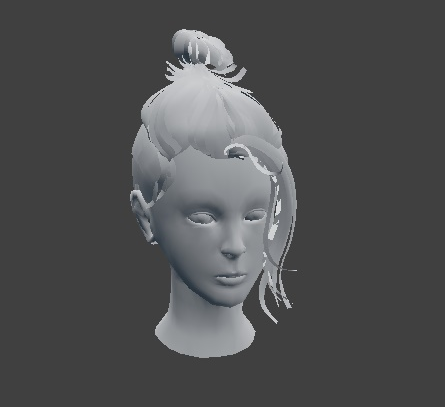
\includegraphics[scale=2]{images/inputHair1}
	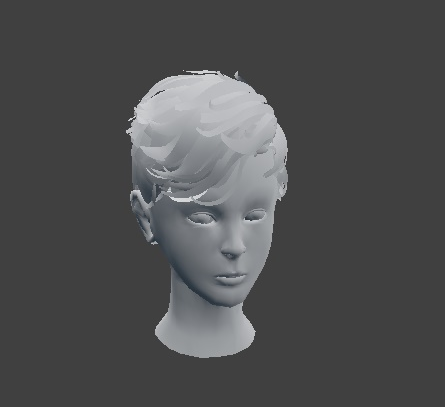
\includegraphics[scale=2]{images/inputHair2}
	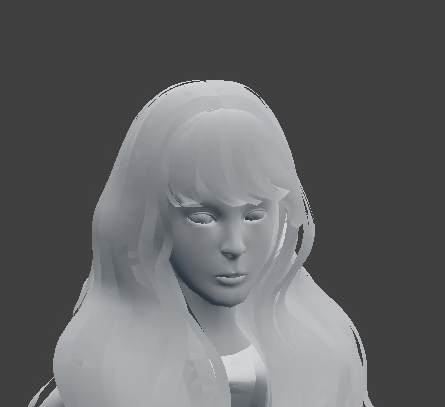
\includegraphics[scale=2]{images/inputHair3}
	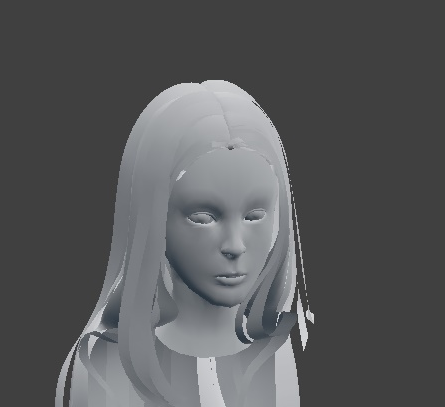
\includegraphics[scale=2]{images/inputHair4}
	\caption{examples of polygon hair mesh training data.}
	\label{inputHairs}
\end{figure}

\subsection{Retopologising Training Data}
\textit{Retopology} is the act of refactoring the topology of a surface into a different arrangement of mesh components. As mentioned, it is often the case for 3D mesh topology to be organised by quadrilateral faces during production. Rendering pipelines convert quad meshes to triangles as an optimisation process. \textit{Simgeom} data are triangulated meshes; reconstruction is performed on all input data to convert the geometry from triangulated meshes to have quadrilateral topology. It is possible to partially automate this process through functionality offered by the Blender API. A script to batch process conversion of multiple meshes executes the following steps in Blender:
\begin{enumerate}
	\item First, a new blank scene is created.
	\item Import a mesh object from the directory that contains the training data set.
	\item Select the imported mesh and enter edit context mode which enables operations for manipulating objects.
	\item Select all vertices of the mesh and apply the \textit{tri-to-quad} conversion operation.
	\item Enter object context mode to export the mesh.
	\item Delete the mesh from the scene
	\item Repeat from step 2 with the next mesh in the training directory until processing of all meshes.
\end{enumerate}

Existing algorithmic solutions for converting a triangle mesh to a quad mesh are imperfect. Remaining triangle faces are required to be removed manually after the procedure. The conversion process alters the geometry very marginally but preserves the representation of hair structure. The quad-faced meshes are used for feature extraction and are assumed to be correct in the context that it is representative of a valid hairstyle. 

\begin{figure}[!h]
	\centering
	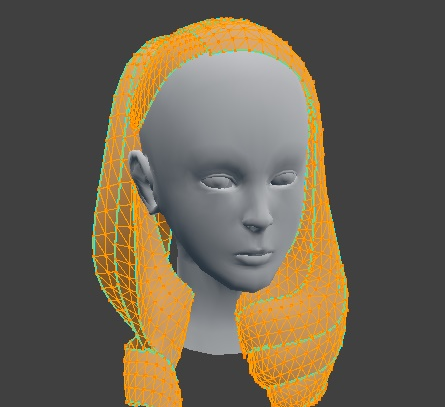
\includegraphics[scale=2]{images/triToQuad1}
	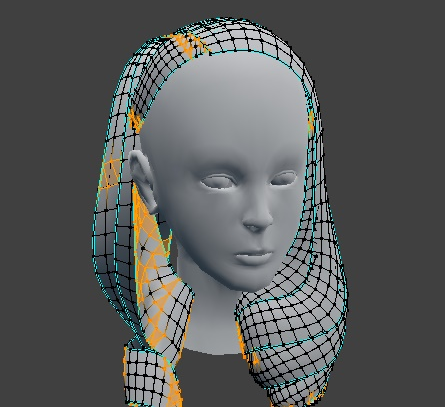
\includegraphics[scale=2]{images/triToQuad2}
	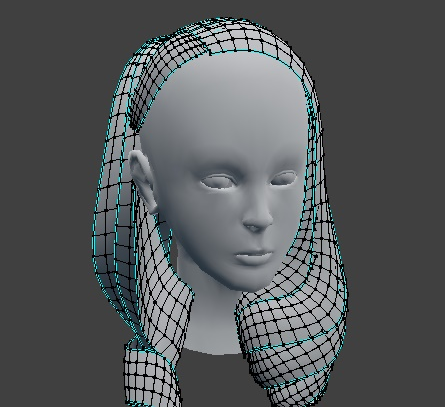
\includegraphics[scale=2]{images/triToQuad3}
	\caption{Triangular faces are highlighted using a selection procedure for all faces that are made of exactly three edges. To the left is an original mesh acquired, the middle shows a selection of remaining triangles after the automatic tri-to-quad conversion, and the right displays a retopologised mesh of entirely quads.}
\end{figure}

Sampling four input mesh from the training set (those displayed in figure \ref{inputHairs}), on average there are around $2 \times 10^{2}$ sub-meshes, $1 \times 10^{4}$ vertices and  $3 \times 10^{4}$ edges per mesh. To retopologise the remaining triangles as quads manually, the hair mesh is separated into individual segments so that visibility of layering sub-mesh surfaces can be toggled to not obstruct vertex, edge, and face components. Each sub-mesh must be inspected to find remaining trianglular polygons. There are many ways one can modify topology of a mesh, we assume that basic methods such as utilising the knife tool or dissolve tool of Blender takes only order of seconds per sub-mesh. The time for manually retopologising a partially converted mesh with the complexity of our training data takes order of hours each. Unfortunately, this meant that it is extremely time consuming to prepare meshes defined by the \textit{Simgeom} format, thus for regression models with larger training sets we settled with including partial examples.

\section{Generative Model of Hair}
To utilise machine learning methods for production of 3D hair geometry,  we develop a generative model of 3D hair structure. Mesh data is tricky to compare as topology and fidelity alter both structure of the data encoded and dimensionality. We address the data alignment problem by approximating the mesh to obtain generative parameters of a similar output possible by a model. Training learns the relation of observed generative parameters obtained from approximating the mesh data.

Wang et al. (2009) parametrised a 3D scalp space using spherical projection\cite{examplebasedhair}. This space approximated the surface of a scalp as a hemisphere with the centre denoting the origin. We apply a similar approach with a spherical coordinate system to determine the surface of a scalp.

The spherical polar coordinate system specifies a point from the origin using three parameters:  $(r,\theta,\phi)$\cite[pp.123-126]{sphericalcoords}. The \textbf{radial distance}, $r$, represents the distance from the origin. We also measure two angles: a \textbf{polar angle}, $\theta$, from the positive $z$-axis (zenith direction) and an \textbf{azimuth angle}, $\phi$, is measured from the $xy$-plane that is orthogonal to the zenith.

\begin{figure}[!h]
	\centering
	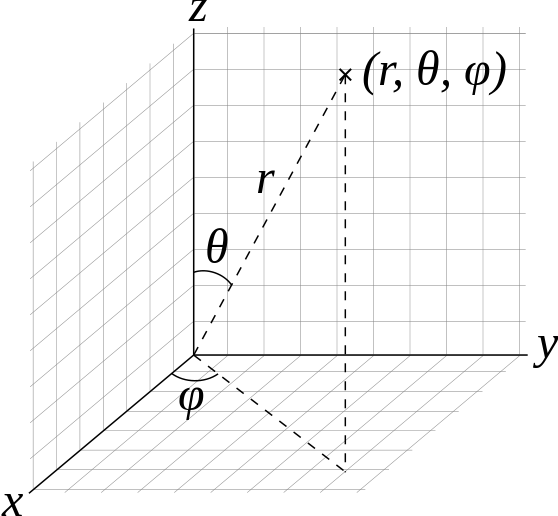
\includegraphics[scale=0.25]{images/sphereCoords}\\
	\tiny{Source: \href{https://commons.wikimedia.org/wiki/File:3D_Spherical.svg}{https://commons.wikimedia.org/wiki/File:3D\_Spherical.svg}, public domain.}
	\caption{3D spherical coordinate system}
\end{figure}

Uniformly placing points at a fixed radial distance and constant intervals within constrained angles give a collection of points that represent hair roots of the scalp. Increasing the number of hair roots allows sampling of higher fidelity. However, this also demands greater computational resources.

\begin{figure}[!h]
	\centering
	\caption{Sphere meshes visualise root positions. The angle ranges specify coverage area of the scalp, while the interval of placements determines resolution. Fitting a sphere to the reference head mesh approximates the radial distance and origin.}
	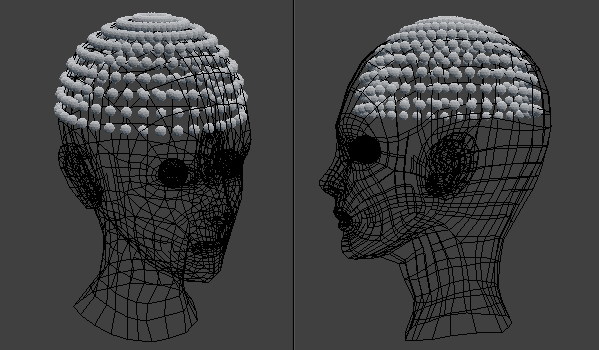
\includegraphics[scale=0.5]{images/spherePoints}\\
\end{figure}

A total of 342 splines in our generative model is used to describe hair structure. We construct each spline from 10 points in a 3D space. The resulting feature vector is 10260 dimensions long.

\begin{figure}[!h]
	\centering
	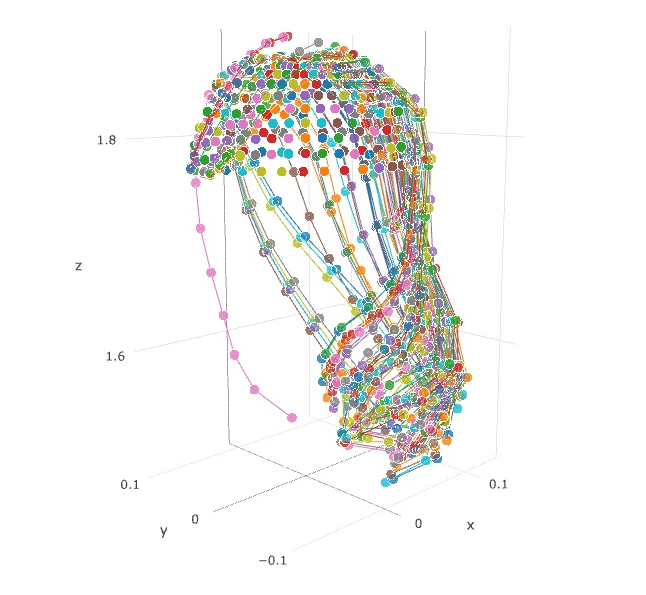
\includegraphics[scale=3]{images/generativeModel}\\
	\caption{A possible configuration of 10260 data points in the generative model}
\end{figure}

\section{Approximating Generative Parameters from Input Data}
\subsection{Parsing OBJ File}
Approximation begins by parsing the geometric data of OBJ files into a graph data structure of nodes and edges. The axis of exported OBJ files is different from the axis of Blender, to align the coordinate system, swap the Y and Z axis, then negate the Y axis. \textit{OBJ} is a human-readable format that declares a mesh element per line. The elements we are interested in are:
\begin{itemize}
	\item geometric vertices, specified by a line that starts with the "v" character, followed by floating values that represent the x, y, z of the vertex position.
	\item face elements, specified by a line that starts with the "f" character, followed by a list of vertex indices that correspond to a vertex line.
\end{itemize}
Variations of the format may exist by implementation, but only the essentials identified are required for our purpose. An algorithm that parses \textit{OBJ} files to retrieve a mesh graph and its corresponding vertex dictionary is given by:

\begin{algorithm}[!h]
	\caption{Parsing OBJ format}
	\algrule
	\textbf{Input}: mesh data file\;
	\textbf{Output}: vertex dictionary of 3D points, mesh graph\;
	\algrule
	\textbf{initialise} vertex dictionary, graph\;
	\For{line \textbf{in} file}{
		\If{line starts with "v "}{
			parse vertex data\;
			add new vertex to vertex dictionary\;
			add new vertex to graph\;
		} \ElseIf{line starts with "f "}{
			parse face data\;
			extract edges from new face\;
			add edges to graph\;
		}
	}
	\Return vertex dictionary, graph
\end{algorithm}

\subsection{Spline Estimation}
\subsubsection{Edge Loop Extraction}
The versatile structure of polygon meshes allows it to be an expressive representation, however, this flexibility can cause ambiguity when analysing geometric structure. We assume that the mesh only contains sub-meshes of hair segments that have grid-like topology. Our assumption allows us to extract edge loops that describe the structure of hair segments. In the technical documentation of Blender, it describes an algorithm for edge loop selection\cite{blenderedgeloop}:
\begin{enumerate}
\item Given a starting edge, only continue searching adjacent edges if the candidates connect to exactly three other neighbours, as any other value would indicate either the border of a mesh or encountering a pole vertex.
\item Completing a cyclic edge loop ends the selection process.
\item Adjacent edges that share a face with the current one are discarded from consideration.
\end{enumerate}
We devise an edge loop extraction algorithm that achieves the properties specified, illustrated in figure \ref{edgeLoopFig}.

\begin{figure}[!h]
	\centering
	\caption{Our edge loop extraction algorithm begins by selecting an edge within the mesh graph. The two vertices of the edge are \textbf{end vertices}. We then proceed to \textit{grow} the edge loop selection. Take the set of \textbf{first degree neighbours} of the \textit{end vertices}, these nodes are the \textit{candidates} for the edge loop. We remove edges that are part of the current edge loop from this set of first degree neighbours. We add the first degree neighbours to a set of face vertices for following iterations. Take the neighbours of the first degree neighbours as a set of \textbf{second degree neighbours}, removing its originating end vertex. A candidate node is only accepted to the edge loop if its set neighbours do not intersect with the set of face vertices. Accepted vertices are appended to the list of end vertices, this process is repeated until there are no end vertices left to grow the selection.}
	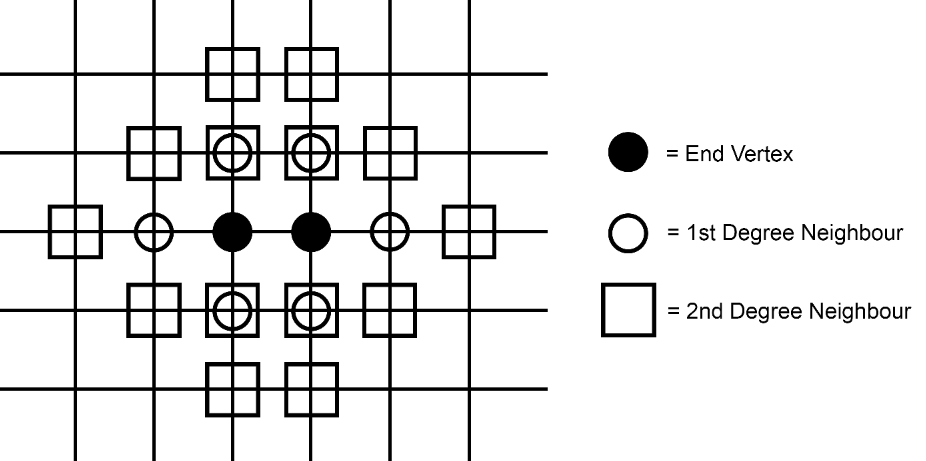
\includegraphics[scale=0.35]{images/edgeLoopDiagram}\\
	
	\label{edgeLoopFig}
\end{figure}

\subsubsection{Boundary and Root Edge Loops}
Hair structure estimation begins by splitting the mesh into sub-meshes, determined by graph connectivity. For each segment mesh, we are interested in the edge loops that represent hair strands from the scalp roots. To find these edge loops, we must locate the boundary edge loops of the mesh and choose one to be the root edge loop.

Corner vertices are nodes that have exactly two edges, while border vertices have three edges. Boundary edge loops are determined by selecting an edge of a corner vertex and growing the edge loop. Any edge of a corner vertex will connect to a border vertex. The selection is specified to stop upon encountering another corner vertex, resulting in an edge loop of the bounds. We discard the vertices of the extracted boundary edge loop. Remove any corner vertices that no longer have any neighbours left in the set of border vertices. Repeat until there are no corner nodes left, thus successfully extracting the boundary of the mesh as a collection edge loops.

\begin{algorithm}[!h]
	\caption{Extracting boundary edge loops}
	\algrule
	\textbf{Input}: vertex dictionary, mesh graph\;
	\textbf{Output}: list of boundary edge loops\;
	\algrule
	\textbf{initialise} corner vertices, border vertices, list of boundary edge loops\;
	\While{number of corner vertices \textbf{in} mesh \textbf{greater than} 0}{
		pick a corner vertex\;
		\For{vertex \textbf{in} neighbours of selected corner}{
			\If{vertex \textbf{in} set of border or corner vertices}{
				extract edge loops\;
				add edge loops to boundary edge loops collection\;
				remove vertices of extracted loops from boundary vertices\;
			}
		}
		\For {vertex \textbf{in} corner vertices}{
			\If{all adjacent border edges of corner vertex have been removed}{
				remove corner vertex\;
			}
		}
	}
	\Return boundary edge loops
\end{algorithm}

\begin{figure}[!h]
	\centering
	\caption{Observe that the corner vertices have two edges, and the boundary edges have three. Determining the root edge loop is done by choosing the boundary edge loop that is closest to the scalp surface.}
	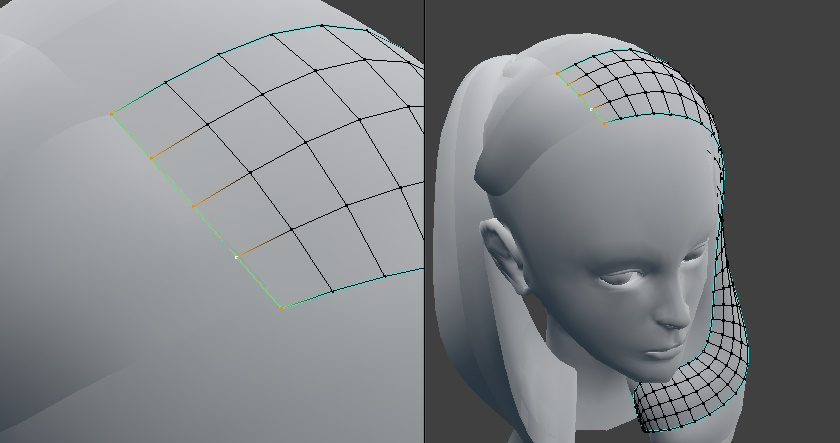
\includegraphics[scale=0.5]{images/rootLoop}\\
\end{figure}

The \textit{root edge loop} is the boundary edge loop that is closest to the surface of the scalp. It serves as a reference for where the hair strands begin. We determine the root loop by finding the average distance of each vertex in a boundary loop. Heuristically, the root border has minimal distance when aligned across the scalp.

There is a significant flaw in this approach as it will not correctly predict roots of hair segments that are represented by multiple meshes. A solution to this would be to accept hair that has clear roots first then iteratively join \textit{floating segments} to the end of the closest corresponding \textit{rooted segment} until there are no more, or the system is unable to connect any segments further.	

\subsubsection{Pivotal Strand Poly-lines}
With the root loop, we can extract a collection of edge loops that represents the \textit{pivotal} (descriptive) hair strands of the segment cluster. Given the neighbours of root vertices, removing the neighbours that are also root vertices will leave edges that represent key strands. When there is one edge, we take the edge loop as a pivotal strand representation. The edge loop will extend until it encounters a pole or ends on the boundary. It is useful to know where the strand starts (from the root), and where it ends. We extract a path from the edge loop graph by continually appending adjacent nodes, starting from the root node. The result forms a spline of connecting lines.

\begin{algorithm}[!h]
	\algrule
	\textbf{Input:} hair mesh\;
	\textbf{Output:} collection of pivotal poly-lines\;
	\algrule
	\textbf{initialise}\;
	\For{sub-mesh \textbf{in} mesh}{
		find boundary edge loops of sub-mesh\;
		determine root edge loop among boundary edge loops\;
		\For{node \textbf{in} root edge loop}{
			\For{neighbour of node}{		
				\If{node \textbf{not in} root loop}{
					grow pivotal strand edge loop\;
					add pivotal strand to poly-line collection\;
				}
			}
		}
	}
	\Return pivotal poly-line collection\;
	\caption{Extracting spline edge loops}
\end{algorithm}

A \textbf{repair operator} processes the strand splines to improve the approximation. First, the starting point of floating splines is attached to the nearest end of a rooted spline, only if there exists one within a specified vicinity. We discard the remaining floating splines that are not attached. Secondly, removing splines that are insignificantly short in length allows for more descriptive splines to be sampled.

\subsubsection{Parametrising a Strand Spline}
The procedure thus far returns a set of strand splines that have varying number of nodes. We produce a constant dimension through sampling to acquire a spline that is applicable for use as parameters of our generative model.

First establish intervals of the distance covered between the points of the original spline. Now suppose we want to evenly sample the spline with $n$ points, we can compute the distance where the $i_{th}$ sample point should travel along the spline as
$$distance=\frac{i \cdot s_l}{n},$$
where $s_l$ is the spline length.

We determine the indices $[j, j+1]$ where the sample distance lies on the spline by comparing the sample distance to the distance of the interval list. The position, $\bm{P}$, of the sample point is
$$\bm{P} = \bm{S} + r\bm{D},$$
where $\bm{S}$ denotes the starting position that is the $j_{th}$ point of the original spline, plus the unit vector direction to the next $j+1_{th}$ point, multiplied by scalar $r$, the remaining distance to cover from the $j_{th}$ interval.

A potential improvement for parametrising the strand splines is to concentrate sampling points at curves rather than evenly spaced. Sampling effectively allows the model to be descriptive with less parameters, mitigating problems introduced by the curse of dimensionality.

\subsection{Structure Estimation}
Spline estimation extracts an arbitrary number of splines. The next step is to choose a fixed number of splines for representing the hair geometry. We introduce a \textbf{selection operator} to associate a root with a spline such that the combination of splines are representative of the hair structure. Attributes that make a spline more desirable to a particular root include:
\begin{itemize}
	\item \textit{proximity} - how close the subject spline is to the root position.
	\item \textit{significance} - how definitive a particular spline is, or the information conveyed by the subjected spline.
	\item \textit{uniqueness} - whether there are other roots that have already captured the information conveyed by the subjected spline.
\end{itemize}
Several selection operators experimented are:
\begin{itemize}
	\item \textit{nearest strand selector} - it naively selects the closest spline of each root position. 
	\item \textit{average strand selector} - picks all strands within vicinity and takes the average representation.
	\item \textit{unique selector} - considers all strands within vicinity and takes the spline that has maximises the minimum distance from any spline already selected by other roots.
\end{itemize}

\section{Learning a Manifold with Bayesian GP-LVM}
Once we have acquired a method to estimate the hair structure of the input data, we can then learn a latent manifold for generative parameters of hair.

A perspective that extends GP-LVM is the paradigm of \textbf{Kernel Method Based GP-LVMs}\cite{reviewgplvm}.  GP-PLVM can be equivalent to \textit{Probabilistic Kernel Principal Component Analysis} (PKPCA) when replacing the $\bm{XX}^T$ term of equation ? with a kernel matrix. The choice of a kernel influences performance of the model as it specifies the prior distribution for regression. Selection of the kernel depends on the task to be accomplished.

\begin{figure}[!h]
	\centering
	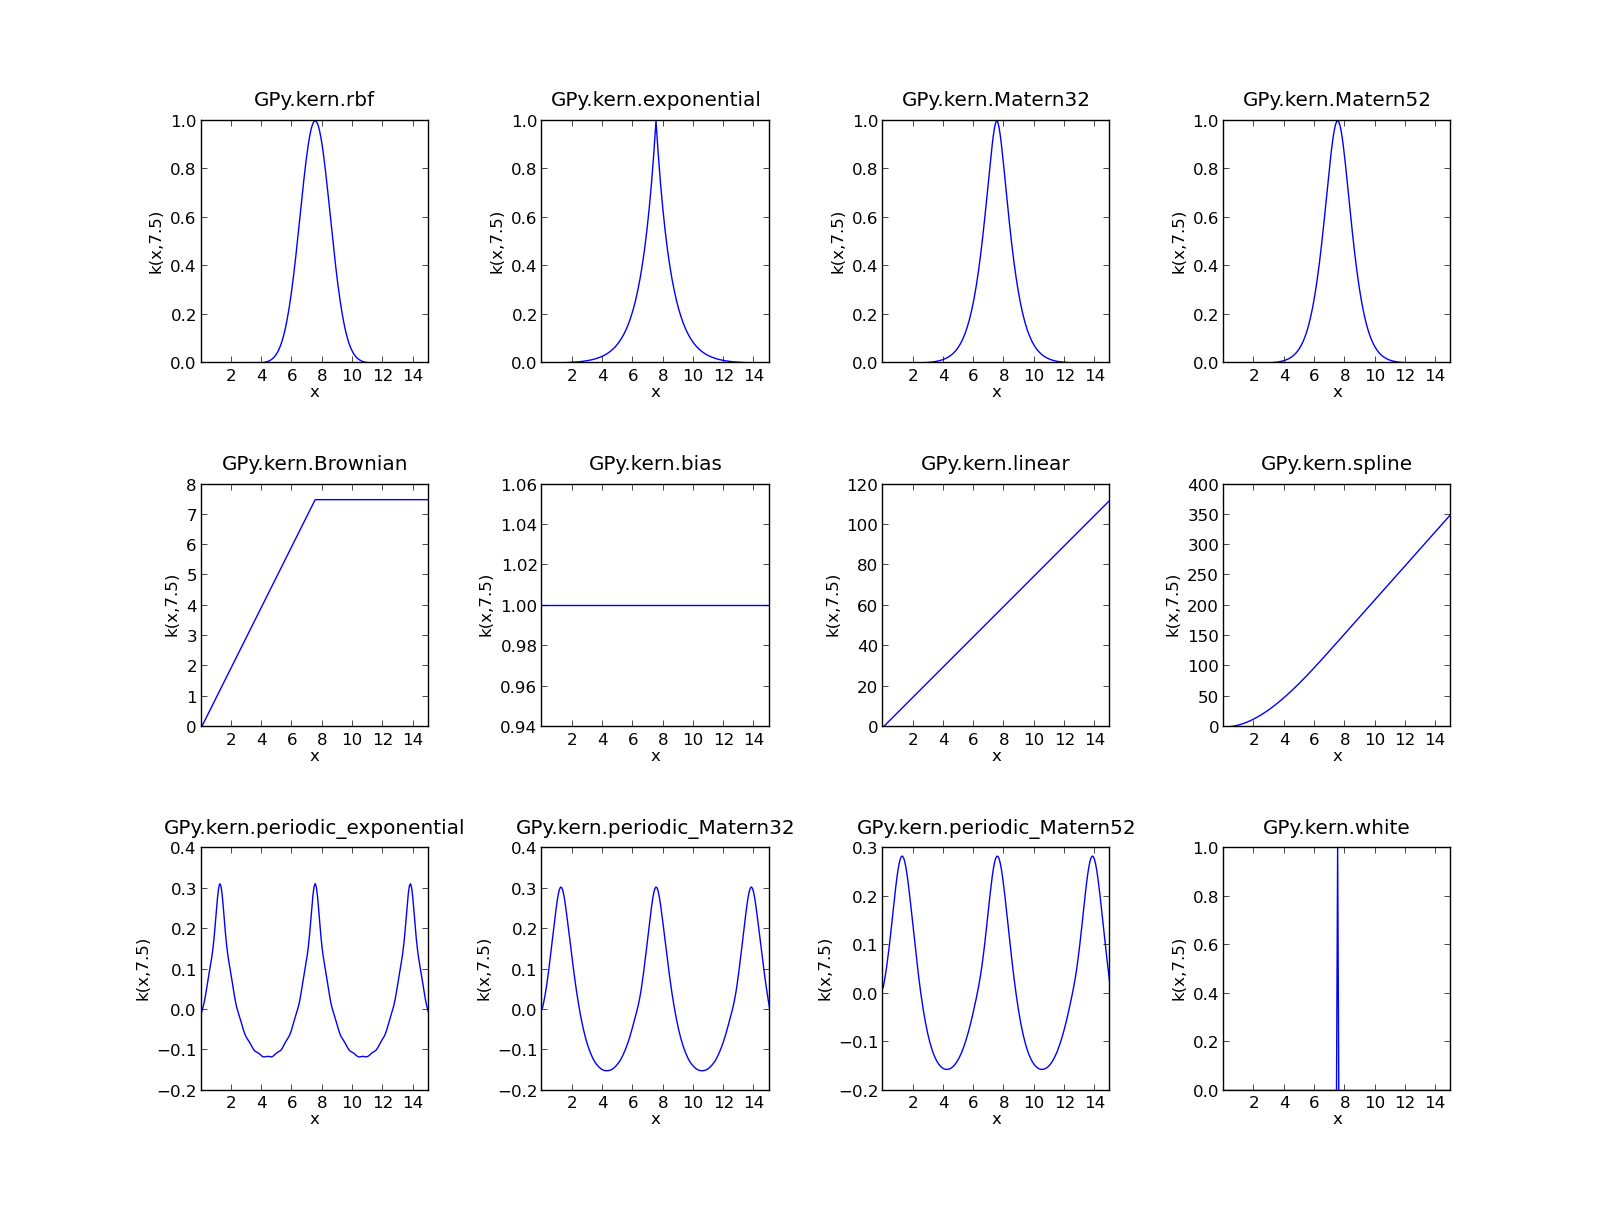
\includegraphics[scale=0.3]{images/gpyKernels}\\
	\tiny{Source: GPy library documentation}
	\caption{GPy offers various standard kernels. Multi-modal kernels can be formed from combining kernels to represent data of complex nature.}
\end{figure}

The \textbf{radial basis function (RBF) kernel} models the data smoothly, interpolating between variables gradually. An \textbf{exponential kernel} places emphasis at peak likelihoods, changing very little from observed data when uncertainty is high. Using a \textbf{linear kernel} is equivalent to modelling with PPCA. Figure \ref{kernelHair} illustrates the results of RBF, exponential, and linear kernels in our regression model.

\begin{figure}[!h]
	\centering
	%\includegraphics[scale=0.3]{images/kernelHair}\\
	\caption{As expected, a linearly embedded hairstyle is of little use as it can only extrapolate along one style. }
	\label{kernelHair}
\end{figure}


\textit{Hyper-parameters} of a kernel specifies its behaviour. A \textit{lengthscale} parameter determines how much the distance of variables influence each other, and the \textit{variance} describes its distribution. We apply \textit{automatic relevance determination} (ARD), which uses the observed data to estimate the length-scale parameters. 

The input data is transformed so that the origin is marginally above the origin of the scalp space. When the regression model is uncertain, it is sensible to bias the prediction towards the mean. Transforming the input data prevents generated hair to move inside the reference head mesh when uncertainty is high. An inverse transformation is applied on the output after prediction so that the generated mesh is located at its intended position. 

\section{Generation of Output}
Completion of the training process provides a regression model that predicts hair structure from estimated input data using our generative model. A problem encountered was incompatibility of the plotting module in the GPy library with the Python distribution of Blender, where a required standard module \textit{TKInter} is not present. To overcome this issue, the training process plotted latent manifold is stored as an image and the regression model is serialised using the \textit{Pickle} module of Python. A Blender add-on implementation can then load the latent manifold image on the UV image editor of the program and through the API, load the serialised regression model to predict latent variables sampled from the manifold.

Output generative parameters are used to create \textit{guide splines} from the poly-line data structure of the Blender API. Polygon mesh geometry is produced from assigning these guide splines to a predefined taper curve and applied with the extrude functionality to create the appearance of hair geometry. An extension to our generative model would be specifying additional parameters such as orientation and width of hair segments, this would enable the regression model to also learn such attributes of the input data.

\begin{figure}[!h]
	\centering
	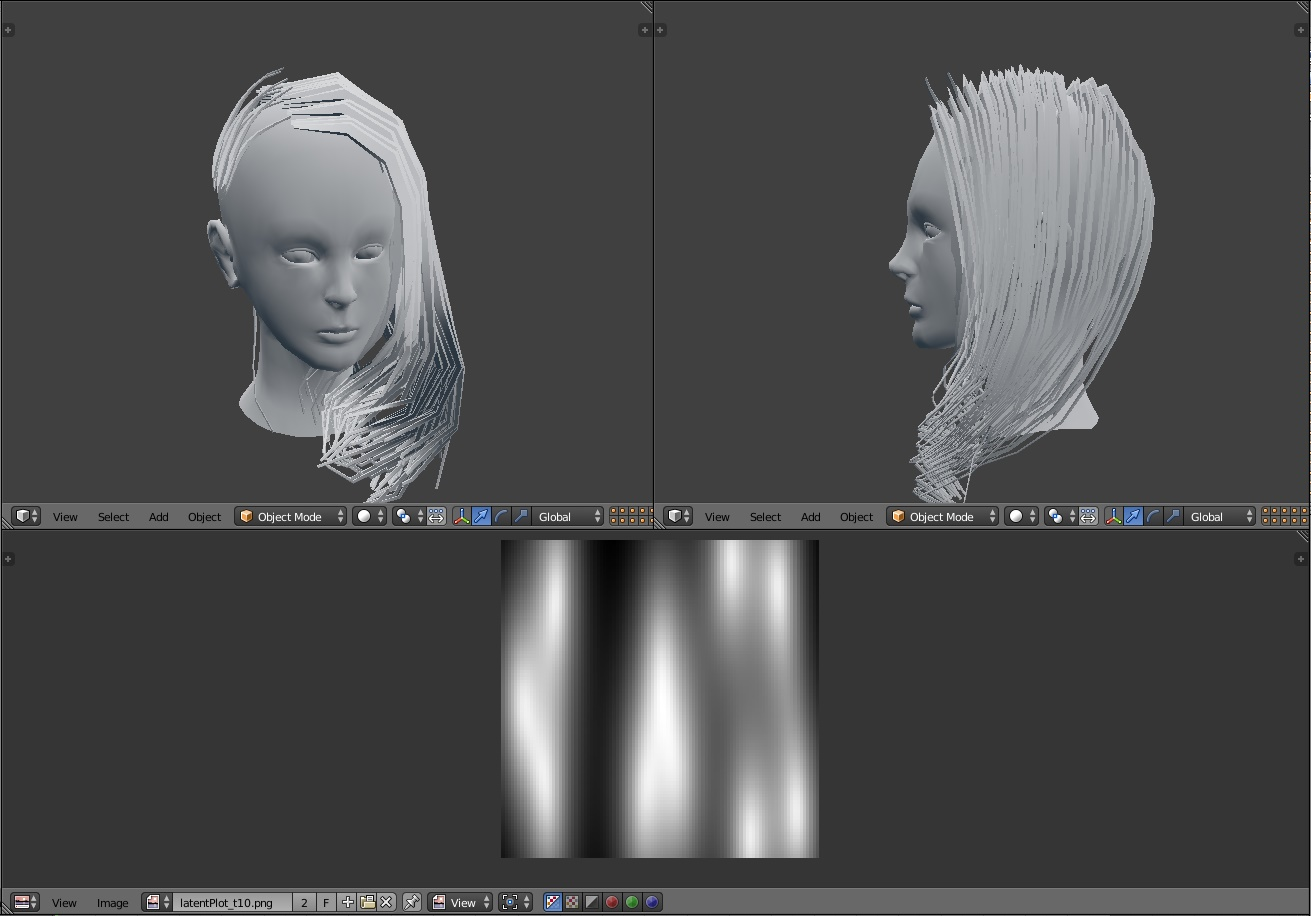
\includegraphics[scale=0.2]{images/latentHairAddon}\\
	\caption{The latent hair modelling add-on for Blender 3D uses the image editor to display the latent manifold.}
	\label{blenderAddon}
\end{figure}


\section{Logging User Activity}
Our add-on implementation can be set to track user activity for acquiring behavioural data when using the latent manifold for geometry generation. Data logged include time spent exploring the manifold, mouse movement, and normalised likelihood of selected predictions. An output management procedure is developed to organise and write logged data automatically so that user testing can proceed seamlessly.

\section{Project Management}
\textit{Git} is used for source control of the project implementation. The branching feature is useful for separating development of features. Maintaining multiple versions of the code base prevented issues caused by the interaction of incomplete features. The merging and rebasing tools helped conflict resolution. Descriptive atomic commits keep a log of progress and supports roll-back to older versions when necessary. A private repository backup was set up on a hosting service provider to prevent data loss and enable development on multiple machines with ease.


\subsection{Time-line}
Calender.
Internal Deadlines.

\begin{table}[!h]
	\centering
	\begin{tabular}{|cc|c|}
		\hline
		foo      & bar      & baz      \\
		\hline
		$0     $ & $0     $ & $0     $ \\
		\hline
	\end{tabular}
	\caption{This is an example table.}
	\label{tab}
\end{table}

Issue tracking was performed on Trello.

% -----------------------------------------------------------------------------

\chapter{Critical Evaluation}
\label{chap:evaluation}
This chapter will start by examining two methods devised to obtain feedback regarding the application of 3D modelling with a latent manifold. First, a survey is used to compare results of the generative output to the training set, and obtain initial reception to the concept. A sample size of 15 subjects completed this survey. Secondly, a sequence of experiments were conducted by users examining our prototype implementation. Activity data was logged to analyse behavioural patterns among subjects. A sample size of 10 completed the experiment. We then proceed to discuss the performance of our demonstrative implementation. The chapter concludes with evaluation of choices made during this project and potential applications of assisted real-time content generation with latent regression models.

\section{Latent Hair Modelling Survey}
The survey starts with a section that queries the name of participants and their experience with producing 3D content. Out of ethical concern, this survey questioned only information necessary for the study, minimising inquiry of personal details. 60\% of the participants considered themselves non-experts, while the remaining 40\% had some form of experience. The first section seeks to evaluate the performance of our generative model. The survey presents participants a series of images consisting of training meshes and meshes generated using the output of our regression model, to which they give a likelihood rating between the range 0 to 10 for which how much the presented geometry resembles hair. 

\begin{figure}[!h]
	\centering
	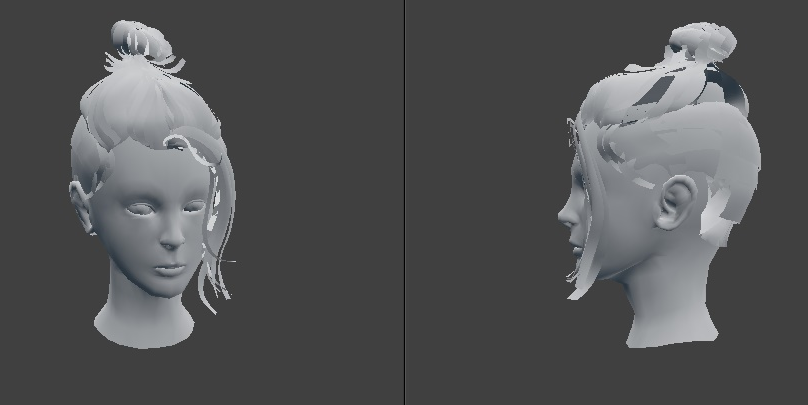
\includegraphics[scale=1]{images/surveyMesh1}
	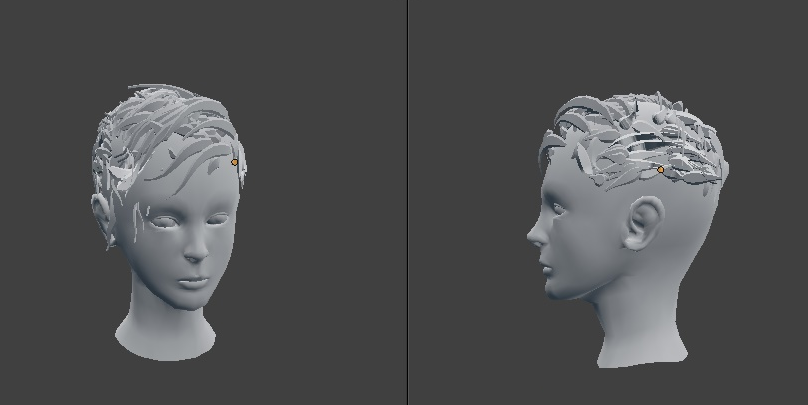
\includegraphics[scale=1]{images/surveyMesh2}
	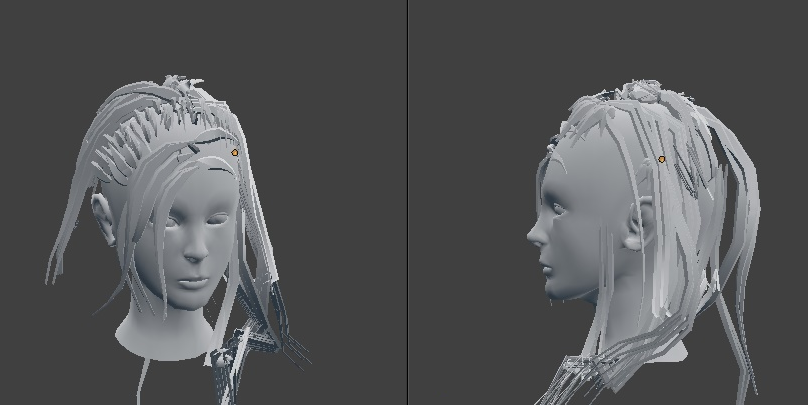
\includegraphics[scale=1]{images/surveyMesh3}
	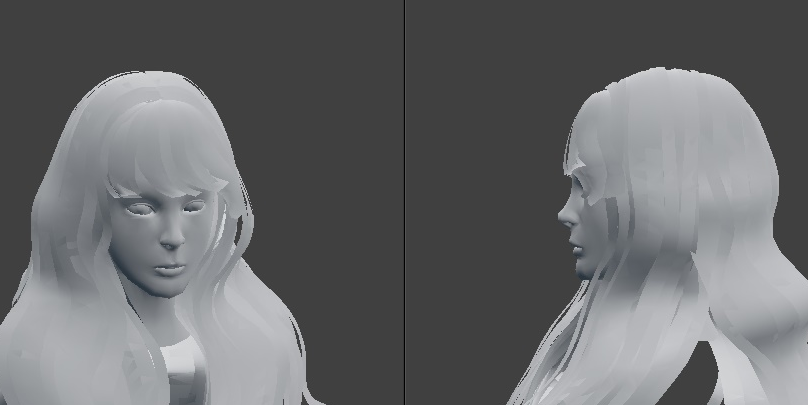
\includegraphics[scale=1]{images/surveyMesh4}\\
	\vspace{0.07cm}
	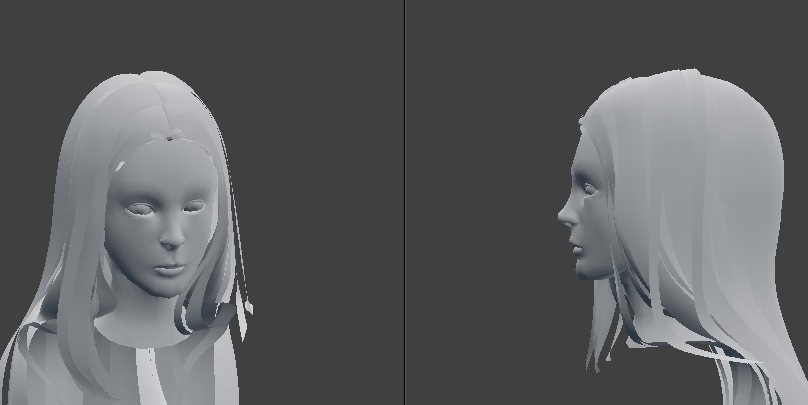
\includegraphics[scale=1]{images/surveyMesh5}
	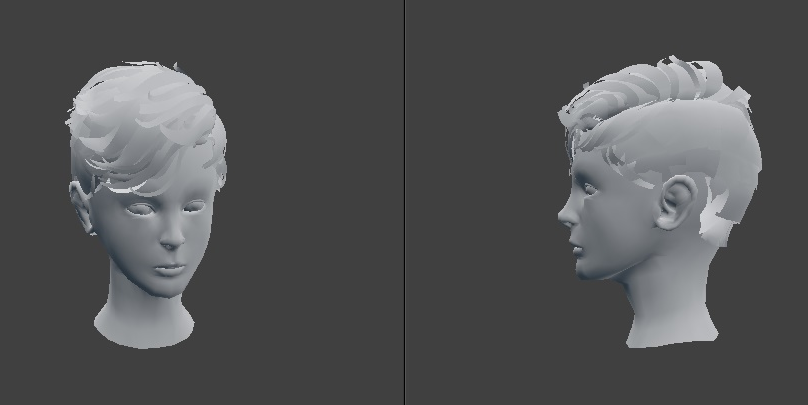
\includegraphics[scale=1]{images/surveyMesh6}
	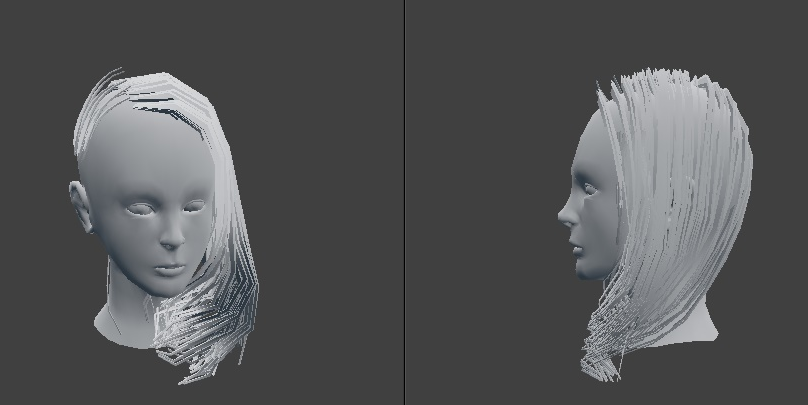
\includegraphics[scale=1]{images/surveyMesh7}
	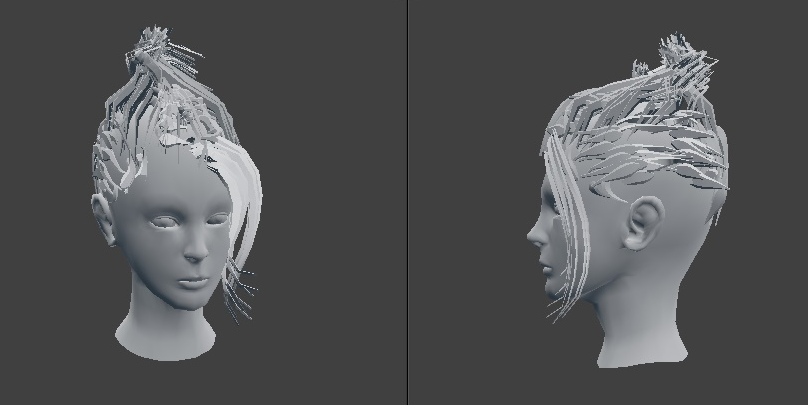
\includegraphics[scale=1]{images/surveyMesh8}\\
	\caption{Images presented in the survey, named mesh 1-4 on the first row from left to right, and 5-8 on the second. Training meshes are 1, 4, 5, and 6. Output mesh are 2, 3, 7, and 8.}
\end{figure}

A mixture of training and output mesh is presented independently without notifying the subjects know which set a particular example belongs to. This enables us to evaluate an objective difference between the perception of training data and output result. If the subject believes that the training meshes are a good indicator for hair, then success criteria for our generative model would be to match those likelihood ratings. Likewise, a low absolute rating for the output mesh is acceptable if the ratings of training meshes are also low.

\begin{figure}[!h]
	\centering
	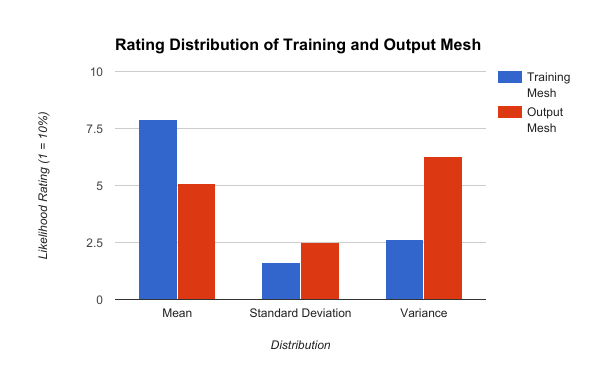
\includegraphics[scale=0.6]{images/meshRating}
	\caption{The mean, standard deviation, and variance comparison of training and output mesh presented on the survey.}
\end{figure}

\begin{table}[!h]
	\centering
	\begin{tabular}{|c|c|c|c|}
		\hline
		Mesh Type 	& Mean		& Standard Deviation	& Variance\\
		\hline
		Training 	& 7.92      & 1.62      			& 2.62\\
		\hline
		Output 		& 5.08 		& 2.51 					& 6.28 \\
		\hline
	\end{tabular}
	\caption{Mean, standard deviation, and variance of training and output mesh (3 s.f).}
\end{table}

In general, training mesh is consistently rated very highly in likelihood at 7.92 mean with 2.62 variance. On the other hand, the output mesh has a mean of 5.08 but results spread out more with a variance of 6.28. To determine whether the difference of results is reliable, we perform an independent samples $t$-test for inferential evaluation. The null hypothesis is that there exists no statistical significance difference between the samples. The $t$ value is computed as
$$\text{t}=\frac{\text{difference between group means}}{\text{variability of groups}}=\frac{\bar{x_1}-\bar{x_2}}{\sqrt{\frac{\sigma^2}{n_1}+\frac{\sigma^2}{n_2}}}$$
We obtain t-value
$$t = \frac{2.84}{\sqrt{\frac{2.62}{60}+\frac{6.28}{60}}}=7.37.$$
The degree of freedom for a sample size of 120 is 118. The test rejects the null hypothesis for a $p$-value of 0.05, where the critical value of a two-tailed test with high degree of freedom is 1.96. This indicates that there is extreme statistical significance between the two sets. From this result, we can infer that there is an observable difference between the training and output meshes.

The following section of the survey introduces basic concepts of 3D modelling and a video depicting the use of a latent manifold for generating meshes. Questions regarding feelings towards use of a latent manifold for 3D production is asked.

When questioned regarding the difficulty of generating output with a latent manifold, the mean is 4.67, suggesting that difficulty is moderate. However, the distribution of responses is skewed, a modal value of 3 tells us that among the sample, most participants found it fairly easy to generate output with a latent manifold.
\begin{figure}[!h]
	\centering
	\caption{Responses for difficulty rating of generating output with a latent manifold, from 1 (easy) to 10 (difficult).}
	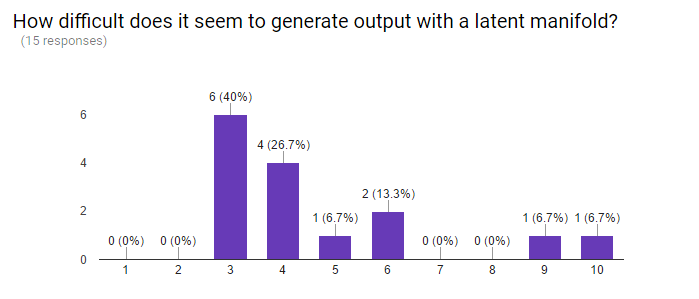
\includegraphics[scale=0.7]{images/surveyDifficulty}
\end{figure}

{\color{red} Calculate quartile percentiles}

The idea of using a latent manifold for exploring new hairstyles or variations of existing ones was welcomed. For exploring styles, the mean is 7.53 with a variance of 2.55, whilst exploring variations have a mean of 7.27 and variance 1.78. In both cases, the high mean value and relatively low variance indicate that participants believe in the potency of discovering new geometry with a latent manifold.

Participants are asked estimate how much of the 3D geometry production pipeline can be automated with a latent manifold. The response resembles a normal distribution, with mean, mode and median at 6, plus variance of 4. 
\begin{figure}[!h]
	\centering
	\caption{Responses for estimation of automating the 3D production pipeline with a latent manifold, from 1 (none) to 10 (all).}
	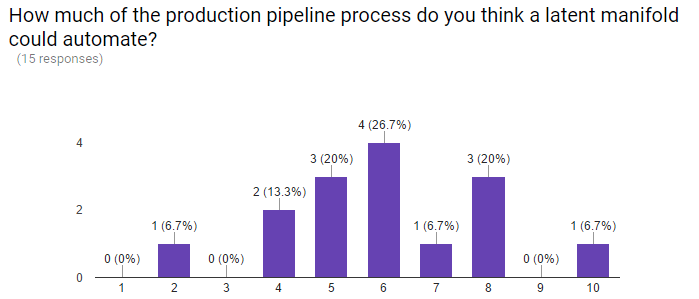
\includegraphics[scale=0.7]{images/surveyAutomate}
\end{figure}

An overwhelming portion of participants are willing to try rapid prototyping with a latent manifold. Out of 15 responses, 6 (40.3\%) participants agreed that they would use a latent manifold for rapid prototyping, 8 (53.3\%) chose \textit{'Maybe'}, and only one participant decided to not use a latent manifold. 

\begin{figure}[!h]
	\centering
	\caption{Responses for whether participants would use a latent manifold for rapid prototyping.}
	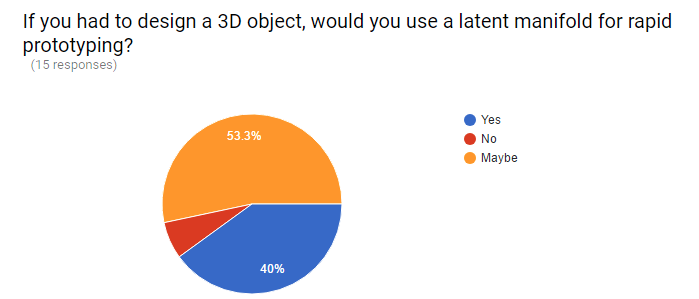
\includegraphics[scale=0.7]{images/surveyPrototype}
\end{figure}

The survey results indicate that whilst the output of our current generative model is notably imperfect when compared to the training data, it is satisfactory expectation as confidence is high in respect to the efficacy of producing 3D content with a latent regression model. Many participants believe a latent manifold is effective for discovering new styles and modifying variations of existing styles. The drawbacks identified include that some users find traversing a non-linear embedded manifold difficult to grasp, thus while it is easy to have an output, controlling the turnout is non-intuitive. That said, most participants would still consider using a latent manifold for rapid prototyping. There is much future research that could yield improved results, to which we will discuss in later sections of this chapter.

\section{Latent Application Experiment}
Participants are shown a series of images from the output of our regression model, displayed in table \ref{experimentmesh}. They are tasked to find the closest corresponding point on the latent manifold that reproduces the geometry presented. An output file with the data displayed on table \ref{outputfile} writes the logged user activity obtained from the tests.

\begin{table}[!h]
	\centering
	\caption{Experiment Geometry}
	\begin{tabular}{|c|c|c|c|}
		\hline
		Test Number	& Image & Regression Likelihood & Manifold Image Position\\
		\hline
		1
					&\raisebox{-.45\height}{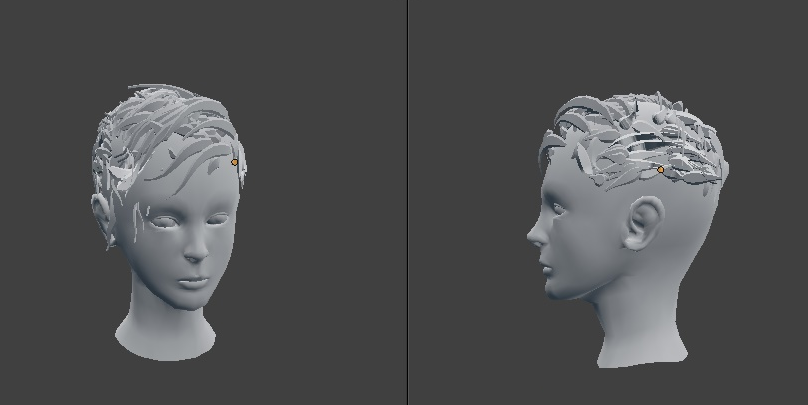
\includegraphics[scale=1.5]{images/surveyMesh2}}
							& 0.929					& 12, 24\\
		\hline
		2
					&\raisebox{-.45\height}{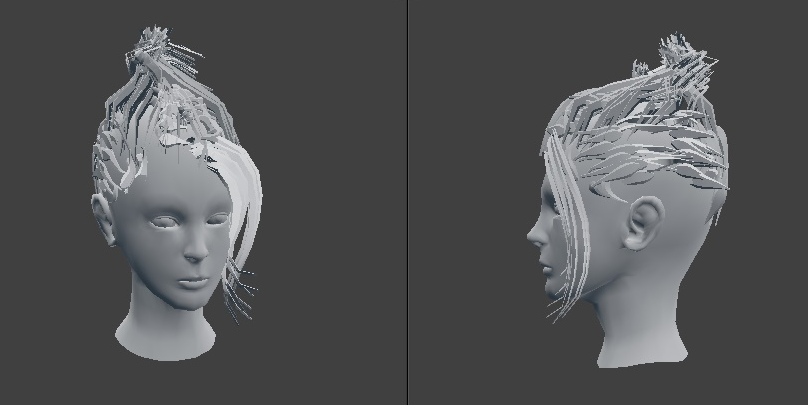
\includegraphics[scale=1.5]{images/surveyMesh8}}
							& 0.925					& 45, 19\\
		\hline
		3
					&\raisebox{-.45\height}{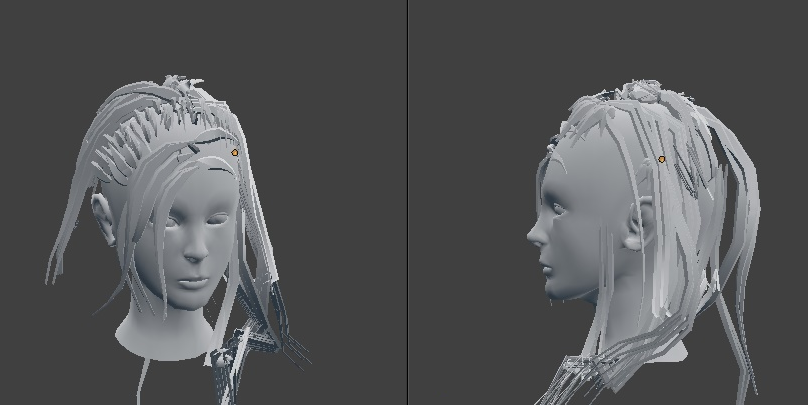
\includegraphics[scale=1.5]{images/surveyMesh3}}
							& 0.902					& 93, 10\\
		\hline
	\end{tabular}
	\label{experimentmesh}
\end{table}

\begin{table}[!h]
	\centering
	\caption{Contents of the output data file.}
	\begin{tabular}{|l|l|}
		\hline
		Data field 				& Description\\
		\hline
		Model 					& The name of the regression model loaded\\
		\hline
		Time taken				& Measure of time spent from starting selection to choosing a result (seconds)\\
		\hline
		Path 					& A list of image coordinates sampled by the cursor during latent selection\\
		\hline
		Distance 				& The total distance traversed by the the path (image pixels)\\
		\hline
		Likelihood				& The normalised probability associated by the regression model\\
		\hline
		Latent Variables		& The selected latent variables\\
		\hline
		Generative Parameters 	& The predicted output of the selected latent variables by the regression model\\
		\hline
	\end{tabular}
	\label{outputfile}
\end{table}

\subsubsection{Behavioural Observation: Familiarising with the manifold}

\begin{figure}[!h]
	\centering
	\caption{Results of a participant who located later targets quickly after spending some time to explore the manifold first.}
	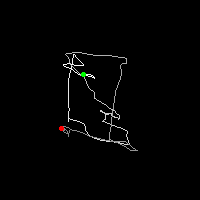
\includegraphics[scale=0.6]{images/experiment/Andrei_ONE_REPLOT}
	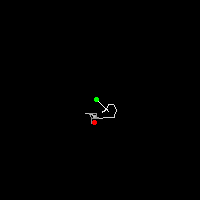
\includegraphics[scale=0.6]{images/experiment/Andrei_TWO_REPLOT}
	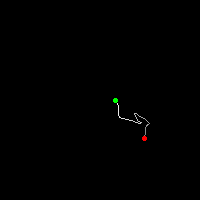
\includegraphics[scale=0.6]{images/experiment/Andrei_THREE_REPLOT}
	\label{andreiresult}
\end{figure}

Some users invest in exploring the manifold thoroughly when first introduced to it. One example is displayed on figure \ref{andreiresult}. After familiarising with a particular manifold, participants are able to locate their objective quickly with improved accuracy.

{\color{red} Back up with stats }

\subsubsection{Behavioural Observation: Fine-tuning the result}

\begin{figure}[!h]
	\centering
	\caption{Plot for the first three tests of a participant.}
	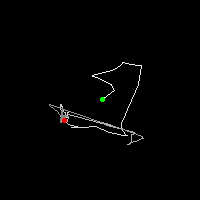
\includegraphics[scale=0.6]{images/experiment/Nick_ONE_REPLOT}
	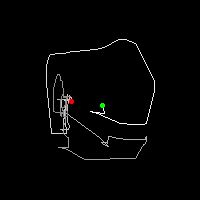
\includegraphics[scale=0.6]{images/experiment/Nick_TWO_REPLOT}
	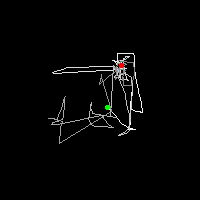
\includegraphics[scale=0.6]{images/experiment/Nick_THREE_REPLOT}
	\label{nickresult}
\end{figure}

Among participants who take significantly longer to select a prediction, some do so as they value precision over speed. Figure \ref{nickresult} shows one such case. We can observe that the participant begins with an exploratory mindset as the path moves boldly, but once they close in to their target, an exploitative strategy is adopted. Staggering movement sets in towards the end of the path as participants attempt to find their best fitting prediction.

\subsubsection{Behavioural Observation: Misleading local optima}

Participants that do not explore the manifold risk becoming stranded within a local optima. Results in figure \ref{mariaresult} is an example of this. The participant did not explore during the first test, which lead to a lengthy search process during the second test - where the participant primarily looked within an area that resembles the target, but the actual target is located elsewhere in the manifold. This is a property that makes the latent manifold unintuitive to use, as it would seem logical for similar meshes to be close in the manifold, but a nonlinear embedding means that this is not always true.

\begin{figure}[!h]
	\centering
	\caption{Plot for the first three tests of a participant.}
	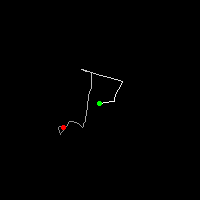
\includegraphics[scale=0.6]{images/experiment/Maria_Marinova_ONE_REPLOT}
	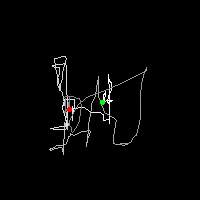
\includegraphics[scale=0.6]{images/experiment/Maria_Marinova_TWO_REPLOT}
	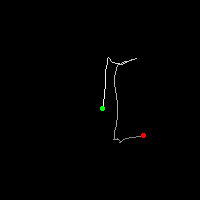
\includegraphics[scale=0.6]{images/experiment/Maria_Marinova_THREE_REPLOT}
	\label{mariaresult}
\end{figure}

\section{Functional Performance}
{\color{red}
	functional  testing, including analysis and explanation of failure cases.
	nice resolution, decent output, measure realtime
	bald spots, inside head, intersection 
	causes and solutions
}

A framework that puts our concept of learning-based assisted content generation to use can be divided into two main stages. First, we have the training process which involves:
\begin{enumerate}
	\item Data acquisition.
	\item Kernel and hyper-parameter selection.
	\item Learning the regression model.
\end{enumerate}
Once a regression model has been trained, it can then be used for production, the regression process that consists of:
\begin{enumerate}
	\item Loading the regression model.
	\item Selecting a latent variable.
	\item Predicting output of selected latent variable.
	\item Generating geometry with predicted output.
\end{enumerate}

The ambiguous nature of creative content and mesh data structure makes training a regression model for 3D content difficult. We have demonstrated how algorithmic solutions can automate the task of preparing input mesh for learning. Content creators that have quadrilateral meshes will not require the retopologising stage, which is necessary for our training set as it contains limiting meshes triangulated for rendering. The unpredictable structure of mesh representation requires making some assumptions regarding the input mesh topology. Despite so, our implementation degrades gracefully with the presence of flawed training data. From edge loops, we determine the structure of the surface.

Training mesh data is scarce. Non-experts content creators are more so susceptible to the lack of training meshes. Learning-based assisted content generation by nonlinear dimensionality reduction is intended to be robust with small training sets. Table \ref{trainingbenchmarks} displays benchmark results of times taken for the training process on our implementation. The benchmark result is highly dependent on many factors including input data, generative model, implementation, and the hardware of the machine. The point to take away is that training a regression model that makes a prediction from selecting variables in a non-linear latent manifold is a reasonably fast, completing in only matter of minutes.

\begin{table}[!h]
	\centering
	\begin{tabular}{|c|c|c|c|c|}
		\hline
		Training Size & Generative Parameters &	Approximation time (s)	& Optimisation time (s)	&	Total time (s)\\
		\hline
		\multirow{3}{*}{10}
		& 2700 	& 100	    & 41     	& 141\\
		& 10200 & 164	    & 49		& 213\\
		& 38850 & 433      	& 86      	& 519\\
		\hline
		\multirow{3}{*}{20}
		& 2700 	& 177      	& 17        & 194\\
		& 10200 & 312      	& 38      	& 350\\
		& 38850 & 877		& 90	    & 967\\
		\hline
		\multirow{3}{*}{30}
		& 2700 	& 265      	& 29      	& 304\\
		& 10200 & 507      	& 65      	& 572\\
		& 38850 & 1321      & 159      	& 1480\\
		\hline
	\end{tabular}
	\caption{Benchmarks of the training process were performed on a machine with an 2.6 GHz CPU (Intel i7-6700HQ), GTX 970M graphics card, and 8GB RAM. }
	\label{trainingbenchmarks}
\end{table}

We use a configuration file to determine properties of our generative model and the fidelity of approximation. In our benchmark tests, we alter the intervals of hair roots to change the number of generative parameters learned by the regression model.

Results of table \ref{trainingbenchmarks} show that approximating generative parameters is the most time-consuming procedure. The time required for approximating is dependent on the complexity of the generative model and input mesh. Thus the benchmark displays a linear relation between total approximation time and training size. Hair geometry as one of the most complicated to be represented use more generative parameters than other categories of surfaces. The number of generative parameters can be kept in sustainable numbers by choice of generative model.

Plotting the latent manifold as a 2D image provides a visualisation of latent variables and corresponding likelihood. Large training sets incorporate more example styles, but too many reduce ease of use as exploring the 2D nonlinear manifold would interpolate unintuitively. Training sets of this solution will inherently be small in cardinality.

A regression model it can be used to predict generative parameters repeatedly. Serialising regression models trained with small sets will result in distributable file sizes. Content creators have the option to collect and share regression models. Refining a GP-LVM regression model is possible by inferring new observations, updating the posterior distribution. The initial time investment required to train a model is made up for if the regression model can reduce total time spent over the course of its usage.

Loading a small regression model and an image is only required once per start-up of a session, and are negligible with contemporary hardware. A 10200-generative parameter regression model on the same machine that performed the benchmark tests spends around $10^{-3}$ seconds to predict an output, using the output to generate hair geometry takes an about of $10^{-1}$ seconds. As a user moves the cursor across the manifold, the implementation presents roughly ten hair meshes per second. This performance is sufficient for producing visible feedback as users traverse the latent manifold.

\section{Evaluative Discussion}
\subsection{Training and Model}
The presence of triangulated faces in training data hinders the accuracy of our regression model. Access to a training set of quadrilateral meshes would improve parameter estimation of our generative model, yielding output that is more representative of training mesh.

The prediction interpolates between styles, drastically differing styles give rise to conflicting substructure of hair geometry. Perhaps it would be more intuitive to use with a training set of varying but similar styles. Campbell and Kautz \cite{fontmanifold} learn manifolds of fonts for individual characters as well as joint manifolds. A single manifold to edit font characters independently allow for more freedom of control. A consideration would be to use a joint manifold for defining an overall hair structure and then refine layers or sections with single manifolds on top. Multiple manifolds divide the problem at hand, reducing outcomes that seem bizarre due to interpolating of non-linear embeddings at the cost of a more preparation required and an involved training process.

{\color{red}
Linear, decision trees, neural nets, GPLVM
Supervised, unsupervised, genetic
Deep GPs and variants
}

\subsection{Comparison with existing solutions}
The AutoHair implementation by Chai et al. (2016) \cite{autohair} delivers hair models that is visually superior in comparison to our demonstrative implementation. AutoHair is a fully automatic procedure, our solution is not intended to replace artists but to assist their creation process. On superior hardware (quad-core Intel i7 CPU, NVIDIA GTX 970 graphics card, and 32GB of RAM), it takes less than a minute for AutoHair to process an image for hair modelling. While this is reasonably fast, our implementation generates geometry at close to real-time. In a production environment, immediate observable feedback is strongly desirable as designs frequently change and creators often want to be directing the progression. 

AutoHair used a database of 300 exemplar 3D hair models and a neural network trained on 50,000 portrait images. The significantly larger amount of material required for the training process increases to the time required for training. According to the originating paper, preprocessing of portrait images is outsourced and takes around a minute per image. The 3D hair exemplars take less than ten hours, and training the neural network is about eight hours. A trained implementation of AutoHair can help 3D artists create models, provided that there is an input image available for the desired hairstyle. It can also be used to discover hairstyles if a 3D hairstyle space is pre-generated. It is unlikely that content creators will collect the material required for training their own implementation. Our solution is more flexible in this aspect, as it expects small training sets. This makes it much faster in performance, while not a fully automatic process, it is suitable for assisted content generation and a strong contender for rapid prototyping. Accepting meshes as input to produce output meshes is also more fitting for a production environment than a portrait image. Our solution can easily be used for different genres of 3D models by specifying a generative model for the type of surface or choosing one of the many existing generative models developed.

Example-based hair geometry synthesis by Wang et al. (2009) \cite{examplebasedhair} is a hierarchical synthesis framework that creates hair models by jointly parametrising hair as a 3D vector field and a 2D arrangement of hair strands. Fully automatic without user intervention. 100,000 strands takes less than two minutes on a 3GHz Pentium 4 CPU with 2GB RAM. The output is textured (texture synthesis), completes more of the production pipeline than our solution. Output is controlled by parameters.
No learning involved, not flexible. Creates novel hairstyles by taking input hairstyle and find statistically similar spatial arrangements of strands and geometric details.
We can use this synthesis framework in place of our generative model.

\subsection{Potential Improvements}
Generative model
Regression model
Simulating foliage, grass.
transferring to fixed objects like a face: mouth, eye, etc that is more "predictable".
Determining threshold of acceptable hair.
As mentioned previously, 3D meshes are delicate and can easily be invalidated from small changes. Thus, reparations to ensure that the output of trained models are acceptable is a topic to explore.

\subsubsection{Addressing Non-Intuitive Use}
Plot small image of output in corresponding area of latent variable model to illustrate the certain areas (training data) so users can explore around it for variation.

\subsection{Applications}
The advent of 3D printing, augmented reality, and virtual reality has resurfaced interest in production of 3D representations. In addition of contribution toward the important production pipeline, content creation extends to consumer applications. Advancements in communication and technology established a culture of creation and sharing experiences on social media. An easy to use method of creating content is a coveted feature.
For example, consider a system in a video game that allows users to create customise their avatar appearance. A content customisation system desires to be flexible, but may be abused to create inappropriate content if no restrictions are applied. This is especially problematic if such content is shared or displayed through an online platform. Our solution can be applied to address this problem training a regression model for parameters of the customisation system and only accept inputs that have an associated likelihood above a certain threshold. Selecting from a latent manifold can update many parameters simultaneously and interpolate between predefined configurations, providing an excellent level of customisation while adhering to defined constraints.

3D latent space with VR.
2 page
% -----------------------------------------------------------------------------

\chapter{Conclusion}
\label{chap:conclusion}

\section{Summary}
(Re)summarise the main contributions and achievements, in essence
summing up the content. 2 pages

\section{Project Status}
Clearly state the current project status (e.g., ``X is working, Y 
is not'') and evaluate what has been achieved with respect to the 
initial aims and objectives (e.g., ``I completed aim X outlined 
previously, the evidence for this is within Chapter Y'').  There 
is no problem including aims which were not completed, but it is 
important to evaluate and/or justify why this is the case. 2 pages

\section{Future Work}
Outline any open problems or future plans.  Rather than treat this
only as an exercise in what you {\em could} have done given more 
time, try to focus on any unexplored options or interesting outcomes
(e.g., ``my experiment for X gave counter-intuitive results, this 
could be because Y and would form an interesting area for further 
study'' or ``users found feature Z of my software difficult to use,
which is obvious in hindsight but not during at design stage; to 
resolve this, I could clearly apply the technique of Smith [7]''). 1 page



% =============================================================================

% Finally, after the main matter, the back matter is specified.  This is
% typically populated with just the bibliography.  LaTeX deals with these
% in one of two ways, namely
%
% - inline, which roughly means the author specifies entries using the 
%   \bibitem macro and typesets them manually, or
% - using BiBTeX, which means entries are contained in a separate file
%   (which is essentially a databased) then inported; this is the 
%   approach used below, with the databased being dissertation.bib.
%
% Either way, the each entry has a key (or identifier) which can be used
% in the main matter to cite it, e.g., \cite{X}, \cite[Chapter 2}{Y}.

\backmatter

\bibliography{dissertation}

% -----------------------------------------------------------------------------

% The dissertation concludes with a set of (optional) appendicies; these are 
% the same as chapters in a sense, but once signaled as being appendicies via
% the associated macro, LaTeX manages them appropriatly.

\appendix

\chapter{An Example Appendix}
\label{appx:example}

Content which is not central to, but may enhance the dissertation can be 
included in one or more appendices; examples include, but are not limited
to

\begin{itemize}
	\item lengthy mathematical proofs, numerical or graphical results which 
	are summarised in the main body,
	\item sample or example calculations, 
	and
	\item results of user studies or questionnaires.
\end{itemize}

\noindent
Note that in line with most research conferences, the marking panel is not
obliged to read such appendices.

% =============================================================================

\end{document}
